\documentclass[conference]{IEEEtran}
\IEEEoverridecommandlockouts
% The preceding line is only needed to identify funding in the first footnote. If that is unneeded, please comment it out.

\usepackage{cite}
\usepackage{amsmath,amssymb,amsfonts}
\usepackage{algorithmic}
\usepackage{graphicx}
\usepackage{float}
\graphicspath{figures}
\usepackage{listings}
\usepackage{textcomp}
\usepackage{enumitem}
\usepackage{caption}
\usepackage{xcolor}
\def\BibTeX{{\rm B\kern-.05em{\sc i\kern-.025em b}\kern-.08em
    T\kern-.1667em\lower.7ex\hbox{E}\kern-.125emX}}
\begin{document}

\title{Concurrent Tree Traversals in Binary Search Trees\\
%{\footnotesize \textsuperscript{*}Note: Sub-titles are not captured in Xplore and
%should not be used}
\thanks{Identify applicable funding agency here. If none, delete this.}
}

\author{\IEEEauthorblockN{Robert Bland}
\IEEEauthorblockA{\textit{College of Engineering and Computer Science} \\
\textit{University of Central Florida}\\
Orlando, FL \\}
\and
\IEEEauthorblockN{Tyler Townsend}
\IEEEauthorblockA{\textit{College of Engineering and Computer Science} \\
\textit{University of Central Florida}\\
Orlando, FL \\}
}

\maketitle

\begin{abstract}
We introduce our reimplementation of what is considered a practical and concurrent binary search tree that maintains logical ordering information within the data structure, but our implementation will be transformed and compared against a transactional data structure. A transactional data structure will be implemented using software transactional memory which provides a system for executing atomic sections of code instead of using locks. This will allow for users to monitor memory locations that threads read and write to.
\end{abstract}

\begin{IEEEkeywords}
Search Trees, Concurrency, AVL, Data Structures
\end{IEEEkeywords}

\section{Introduction}
%Introduction should state the problem at hand and give some background %information and more about the progress and correctness. 
%Define and explain our topic as well the transactional data structure.
%Transactional data structure are

Concurrency is rampant in today's programming society and we are quickly adapting all serial data structures into concurrent data structures to actually benefit from our ever increasing core count of our CPU's. This now leads into our topic which covers two important and well known data structures, which are Binary Search Trees (BST) and Adelson-Velskii and Landis Trees (AVL). A Binary Search Tree is a node-based data structure that has a root that is the top of the tree and has two subtrees, which are the left and right subtree. The left subtree contains all nodes smaller than the current nodes key and the right subtree contains all nodes with keys greater than the current nodes key. An AVL Search tree is a modified BST, but now we also keep track of heights of all nodes, so that the left and right subtree height don't differ by more than one. If the differences between the two subtrees are greater than one then we rebalance the trees to keep the heights within that range to speed up our search time. The two trees must maintain two rules for our concurrent implementation, the first rule is that it cannot contain duplicates and the second rule is that it has to follow the standard BST/AVL structural layout.
	A potential problem is presented when implementing certain methods concurrently. Some questions that are brought up would be when to lock, the locking order and how can we implement a contains that is exceptionally fast and lightweight, since contains is typically called the most out of any method. Even with all this in mind the main question that hasn't been asked is now being answered, which is how do we generalize an implementation such that it can be applicable to any search tree and not just create specialized solutions [1]? The answer to such a practical search tree is one that introduces a condition for path traversal validation, such that it is applicable to any tree. The condition determines whether or not our key is in the tree by looking at the succinct path snapshot (SPS) and the traversal only needs to take a path limited by our succinct path snapshot. If the key is contained in one of the snapshots then the condition states that the key is in the tree otherwise it states that it does not exist in the tree.  Also, our snapshots will get modified if there are any changes or mutations to the tree or along a path. Using this idea of succinct path snapshots we can also extend it and create a lock-free implementation of contains since it now has a method to verify if our path has been modified without the need to traverse the tree again. This contains however, will traverse again if the verification method fails and because of this it cannot be wait-free since it could fail an indefinite amount of times (Sec 3).
	Our path condition also makes it possible to extend our implementation to allow for customized operations, such as rotations, without having to complicate our program any further. This will prove to be incredibly useful because one of our goals is to recreate our program to be a transactional data structure. A transactional data structure focuses on atomicity and on isolation to ensure that each action takes effect in sequential order.

%\section{Research}
%The research in this area, so compare to other papers?

\section{Implementation}
In this section we will be going over what each function does and describe the linearization points of each function (excluding TraverseNLock). We will also mention progress guarantee, correctness condition and synchronization techniques (NOTE: Maybe move this technique idea to design). The functions to be described are Contains(), Insert(), Remove(), UpdateSnaps() and TraverseNLock(). We will also describe how we initialize our tree and our sentinel nodes. Important note is that every node has an atomic mark designating whether or not it has been logically removed.
\subsection{Tree and Nodes}
Our tree implementation is very familiar if one has seen a standard BST tree, since items less than the current key go down the left path and items greater than the current node go on the right path, but one core idea that our tree follows is that we can only add nodes at the end of the tree and not in between two nodes. We can still remove nodes anywhere in the tree and in one scenario we will actually swap nodes, but for more information on that check the Remove() section. Our tree is initialized to have two sentinel nodes to handle edge cases and the first item we insert will become the root. Our nodes implementation for our concurrent method is different then what we had for our serialized implementation and it will look like this :
\begin{enumerate}
\item T Key
\item Atomic Snapshot (consists of two nodes)
\item Node* LeftChild
\item Node* RightChild
\item Node* Parent
\item Height (For AVL)
\end{enumerate}
We must also keep track of our parent so that we can traverse up the tree when doing certain methods and to help maintain our locking-order, discussed in design decisions.
\subsection{Snapshots}
Snapshots are an integral part of our design because it will guarantee that our contains will not miss any elements that have been moved since it has started. We implemented it by having each node contain a succinct snapshot that contains itself and its successor or predecessor[2(Power Point Slides One)]. This will create an implicit list of nodes with keys in ascending order, note that it isn't linked so we cannot traverse through that list with our contains. We do not search through this linked list, but if the item is not within that list then we can say that it does not exist.
\subsection{UpdateSnaps}
The UpdateSnaps() function called by Insert() or Remove() to update the succinct snapshots of every node that has been changed by the that Insert() or Remove() call. UpdateSnaps() takes one of the following as its parameters:
\begin{enumerate}[label=(\roman*)]
	\item A Node
	\item A Node plus condition
	\item Four Nodes
\end{enumerate}
(I) is used only for Inserts() since we only care about changing that, Remove() will call (II) if the left and right node are leaves or if the right node is its successor and (III) is called when the node being removed has two children and its right child has left child, which will be our nodes successor. This function is recursive and locks nodes if Remove() has called it to change the parents succinct. 
\subsection{Contains}
The Contains() function that we have developed has to be lock-free or there was no point in recreating this paper, so when we develop it we can only use compare-and-swaps. Knowing this we have developed it to at most only use one compare-and-swap, which will be used if we do not find the item. Our contains will have two scenarios happen, either the item has been found when we traverse from the root with our key or we have reached a leaf and cannot find the item.
Our implementation has a lock-free contains and a deadlock-free insert and removes. Our contains() is lock-free because it only uses compare-and-swap, which has a consensus number of infinity, so by only using that atomic operation in that function we can say that even if it fails at least one other operation managed to succeed. If we find our item/key at a node in the list then we check if has been logically removed with a marking on that node and if it not marked then we return true otherwise we restart. This trait proves that this implementation is not starvation-free so it is not wait-free as well. If Contains() could not find the item/key then it reads the succinct snapshot of the node and checks whether or not it is contained in that snapshot. If it is then that means the node has been swapped out and it will restart to find it otherwise we return false.
\subsection{TraverseNLock}
TraverseNLock() will lock the node we are trying to find or a leaf in the tree, if we didn't find our key. Our implementation is identical to Contains() except that it contains locks and returns our node that is now locked instead of a boolean. There are two possible places that we lock, the first being right after we check the marking of our item/key if we found it. The second possible place to lock our node is right before reading the succinct path snapshot to guarantee, which will guarantee that no contaminated data in the set if we do it here.
\subsection{Insert}
A concurrent insert is very similar to a sequential insert with the only difference being that we need to update our snapshots. Our insert first starts by taking in a key and uses TraverseNLock, which returns a node that we locked, to find out where our key belongs. If this node is our key then we unlock the node and return false since we do not allow for duplicates. If we didn't find our key then the node locked will be our parent and we will create a node that contains our key. We then set the parent point of the newly created node to our locked parent node. We then set our parent nodes left or right node pointer, depending on whether or not our key is less than or greater than our parents key, to our newly created node. Then we update the snapshots of our newly created node, unlock our parent node and finally returns true.
\subsection{Remove}
A concurrent remove will take in a key k to remove from our tree and if it returns false otherwise it returns true. First remove will find and lock the node containing our key using TraverseNLock. If we didn't find the node containing our key then we return false.Then it follows one of three scenarios
\begin{enumerate}
\item If the locked node has one child then we first mark the node as removed, which is the linearization point, then we update our snaps, unlock all the nodes it locked and returns true.
\item If the locked node has two children and our right child has no left child then first mark the locked node as removed. Then we set our parents right node to be our right child and our right child will point to our left child, then we update snaps, unlock all the nodes it locked and returns true.
\item If the locked node has two children and our right child has a left child, we first mark our node for removal. Then we have to traverse through the tree and attempt to lock our successor, which restarts when it fails. If we successfully lock our successor then we lock the successors parent to change its left pointer to the successors right child, if it has one. We then swap our successor and locked node, update snaps, unlock all the nodes it locked and returns true.
\end{enumerate}  
\section{Design Decisions}

%locking-order

%TALK ABOUT HOW WE DIDN'T USE A LIST FOR SNAPSHOTS

%TALK ABOUT WHY WE LOCK BEFORE THE READ

%Locking Order as well

We designed our implementation to mirror the pseudo-code of the paper in [1]. This came with benefits of being able to efficiently program and recreate most of what the authors intended for us to implement. However, there were also some challenges as well since they intentionally left out where to include some locks in the pseudo-code and omitted some parts of the code for updating our snapshots. They did mention the potential location of each lock or where certain critical sections are with respect to the pseudo-code and presented some locations for putting locks in the insert and removal implementations. By leaving out some locations this give us enough leeway to interpret when we should use locks in our UpdateSnaps() function, but we have to implement to maintain correctness for our algorithm.
	One common problem when designing concurrent structures is addressing deadlocks and preventing such scenarios from happening. First we should expand on what a deadlock is. A deadlock occurs when one thread locks a resource and needs another resource that another thread has locked and that other thread also needs the first threads resource before unlocking its own resource. This creates a cyclic dependency and thus we can say that that algorithm is prone to deadlocking. We solve this problem by implementing a general locking order that all methods will follow. When traversing we will lock from the bottom-most leaf and work up the tree. When we break this ordering, by locking a node that isn't a leaf, we will attempt to lock nodes below us, so that if it fails we will release our lock. If we didn't release our lock on a failed attempt then we will create this cyclic dependency mentioned earlier and create a deadlock scenario which will ruin our correctness condition.
	Linearization is important when mentioning the correctness condition of our algorithm. So a linearization point is the point in time, usually a line of code, when a method/function operation can be seen by other threads. In the case of adding we say that the linearization point is when our node is reachable from our parent that we added ourselves to. A remove is linearized once we mark our node for removal. Contains has two linearization points however, the first linearization point of contains is with respect to a remove and its a race to see who can read or mark the node they are searching for. The second linearization point is when the node isn't found and we check the atomic snapshot. Since the snapshot can possibly be modified by a remove or add before we check that snapshot, so if we check that and we cannot find our key in that snapshot then we can say that the key isn't in the list and can return false.

\section{Transactional Memory}
Software transactional memory which provides a system for executing atomic sections of code instead of using locks. This can prove to be useful at times and there are various reasons why it is used. The type of software transactional memory that is used is GNU Compiler Collection (GCC) transactional memory. There are reasons for using this, but more importantly this section covers what GCC transactional memory is, how it is implemented and why it was used in the implementation.
\subsection{What is GCC Transactional Memory?}
GCC transactional memory is used to create blocks of code that will be executed atomically. This is to provide programmers with an easier tool to use for concurrent programming when compared with locks and the use of atomic primitives \cite{b4}. It uses the idea of the code blocks to make the idea of where an atomic transaction begins and ends an easier concept as well. Everything inside of the block of code will also be executed in an all or nothing fashion, so if another transaction block (or thread) causes a conflict on a memory access with the current block then we abort and rollback all modifications and try the transaction. This transactional memory also has specific properties associated with it as well that can be applied to any variable or function. The two properties are defined as transaction safe and transaction unsafe. For the transaction unsafe property, it is assumed if the code has or contains the following \cite{b4}:
\begin{itemize}
\item it is relaxed transaction statement (we don't use this)
\item it contains an initialization of, assignment to, or a read from a volatile object
\item it is unsafe asm declaration
\item it contains a function call to a transaction-unsafe function, or through a function pointer that is no transaction-safe
\item it has a volatile variable (so no atomic or volatile variables)
\end{itemize}
The transaction safe property, however, will be allowed to execute inside the atomic block of code if it isn't declared transaction unsafe. There are even more rules to what is exactly transaction safe and unsafe, but that is very complicated and some irrelevant, so a reference is provided for knowing more about this \cite{b4}.
\subsection{How is Software Transactional Memory it Implemented?}
Implementing GCC transactional memory was straight forward due to the simple nature of its calls. Typically, the implementation involves creating the working sequential version of the data structure, then modifying it by surrounding code that will be shared or expected to be modified by other threads in a transaction atomic block. The sequential version of the GCC transactional memory implementation used this style, but in a very broad sense. The sequential implementation involved the removal of all atomic wrappings, so no atomic variables, and the removal of all mutexes, so removing all locks and unlock calls from the code as well. These two actions plus inserting a transactional block of code for all of our function lead to the following sequential implementation for insert:
\begin{lstlisting}
void SerialStmBst::insert(int const &data){

  // Otherwise we traverse
  while (true) {
    __transaction_atomic{
      //Do insert function
      ...
      // AVL Rotations
      if (isAvl) rebalance(curr);
    }
  }
}  
\end{lstlisting}
Implementing the most basic form of transactional memory was simple and straight forward, but increasing the performance was tricky. The actual increase of performance then comes from checking what sections of code doesn't need to be included inside the transaction, so that the transactions are smaller. It is implemented such that the transactions are light weight to ensure that when a transaction does fail it won't have to retry more code than it has to. The improvements made to the original implementation was removing transactions from contains and traverse since they do no write operations. Another change made was to decouple the traverse from the insert and remove. This small change made it, so the implementation doesn't have to retraverse the tree. Some checks have been inserted as a result to ensure that the current node that is being worked on is still a valid option. Another modification made to increase performance was the decoupling of rebalance from insert and remove to increase performance of AVL tree operations. Before it would
\subsection{Why Use Software Transactional Memory?}
The main purpose of using this transactional memory is to remove complexity of locks \cite{b4}. The management of what thread has what lock and whether or not a mutex is held by a thread based on some conditionals is the reason why it is even considered. In the implementation that was done, to transform the remove function from a behemoth of locks, in which each thread had to keep track of up to eight different locks, instead into a block of atomic transaction just by surrounding the block of code and removing any use of locks or unlocks. The price to pay, however, is very steep since the performance will be significantly lower since threads will now waste cycles trying to perform these transactions. Balancing the usefulness of the simple resource sharing and performance is a hard task and the transactional memory implementation emulates just how much has to be sacrificed for reduced complexity. The other purpose of transactional memory is to significantly lower the possibility of data races and deadlocks \cite{b4}. Data races are a serious problem that can cause unexpected behavior which leads into an exorbitant amount of security risks. Also, deadlocks are a plague to all parallel programmers since they often don't immediately take effect and happen in very niche scenarios. Those headaches are mostly alleviated with the use of transactional memory since it will make it far easier to see where the problems occur since all code within transactions are all or nothing, so it isn't possible for one transaction currently making a change to cause a data race or deadlock with another making a change to the same variables.
\section{Performance Evaluation}

Testing the implementation was done on TODO:PUT TYLER PC SPECS HERE. It should be noted that the performance is expected to significantly decrease across all platforms when the number of threads increase past four because of hardware limitations. The concurrent data structure is expected to do significantly better than the software and improved software data structure because of how transactional memory operates. The number of benchmarks was three and those three were:
\begin{itemize}
\item 9\% Insert, 1\% Remove, 90\% contains
\item 20\% Insert, 10\% Remove, 70\% contains
\item 50\% Insert, 50\% Remove, 0\% contains
\end{itemize}
\subsection{Concurrent Data Structure}
The results for the concurrent data structure came out as expected. The AVL tree outperforms BST in most scenarios because of how fast read operations are in AVL trees due to their balancing. For example, BST could have a one long branch that extends for hundreds of nodes, but an AVL tree will not suffer from this and will ensure that there are no left or right heavy sub-trees. Where the performance decreases is when rebalancing will get called more often and cause threads to lock nodes that other threads require. Another possible reason why the performance starts to equalize around 50\% contains and removes is because of how costly it is to remove non-leaf nodes. Any leaf node will require at most two locks, while removals of non-leaf nodes could require up to eight locks! In BST's the removal and adds have a much higher chance of creating leaf nodes and the number of lead nodes in AVL tree is significantly lower due to rebalancing. The performance for 50\% inserts and removes perhaps show that there are better alternatives if the user requires a tree to do very minimal amount of inserts. However, if the user needs a light weight contains function then these graphs prove that it is possible to get up to ten million operations per second with only four threads!
\subsection{Software Transactional Memory Data Structure}
The software transactional memory data structure performed better than expected since the description of this data structure creates a deceptive idea that using it means very little concurrency, and in one scenario it was superior than the concurrent data structure. The transactional data structure BST implementation outperforms the concurrent data structure with the 50\% remove and insert benchmark. This indicates just how costly it is for removes in the concurrent data structure implementation if a transactional data structure could beat it. Again, the reasoning for this difference is because of how costly remove can be inside of the concurrent data structure. The decrease in overall performance from our data structure comes from how it operates, since adds will conflict with each other often and force a complete restart rather than a normal check. Since adds are very light weight in the concurrent data structure with only one lock, it hurts performance for a transaction to have to completely restart while an add
\subsection{Improved Software Transactional Memory Data Structure}
The improved implementation of software transactional memory data structure has surpassed the original implementation with only a few changes. These changes, as previously stated, has lead to an overall increase of at least 10\% with numerous 50\% increases. There were expected increases in performance due to the number of transaction conflicts decreasing. Decreasing the amount atomic block of code for a transaction does increase performance. Decoupling the rebalance and traverse has greatly increased the AVL's performance especially when using more threads because with four threads it experiences a 50\% speed-up when compared to the original transactional memory data structure implementation. However, even with all of the improvements that have been made to the transactional data structure it still does not out perform the concurrent data structure on two benchmarks.

\begin{figure*}[ht!]
%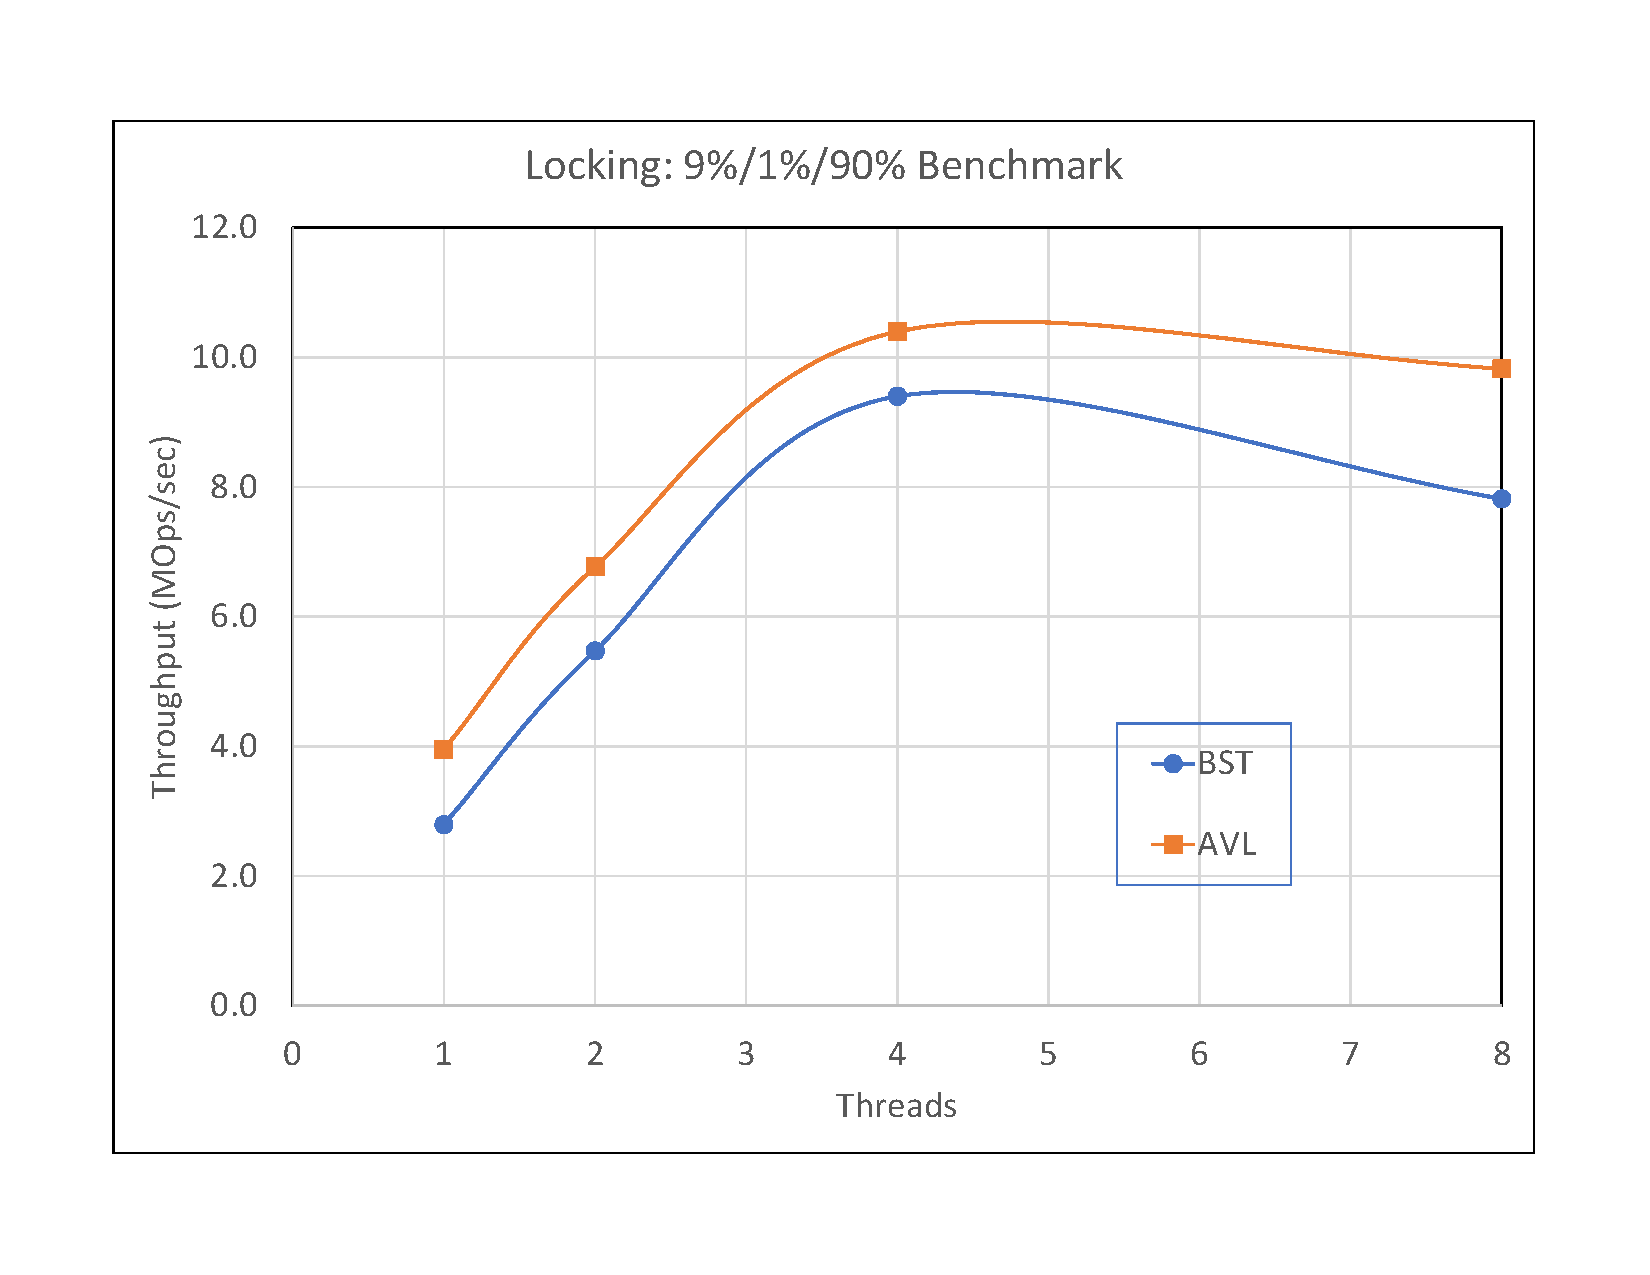
\includegraphics[width =.3\linewidth]{figures/conc-9-1-90}\hfill
%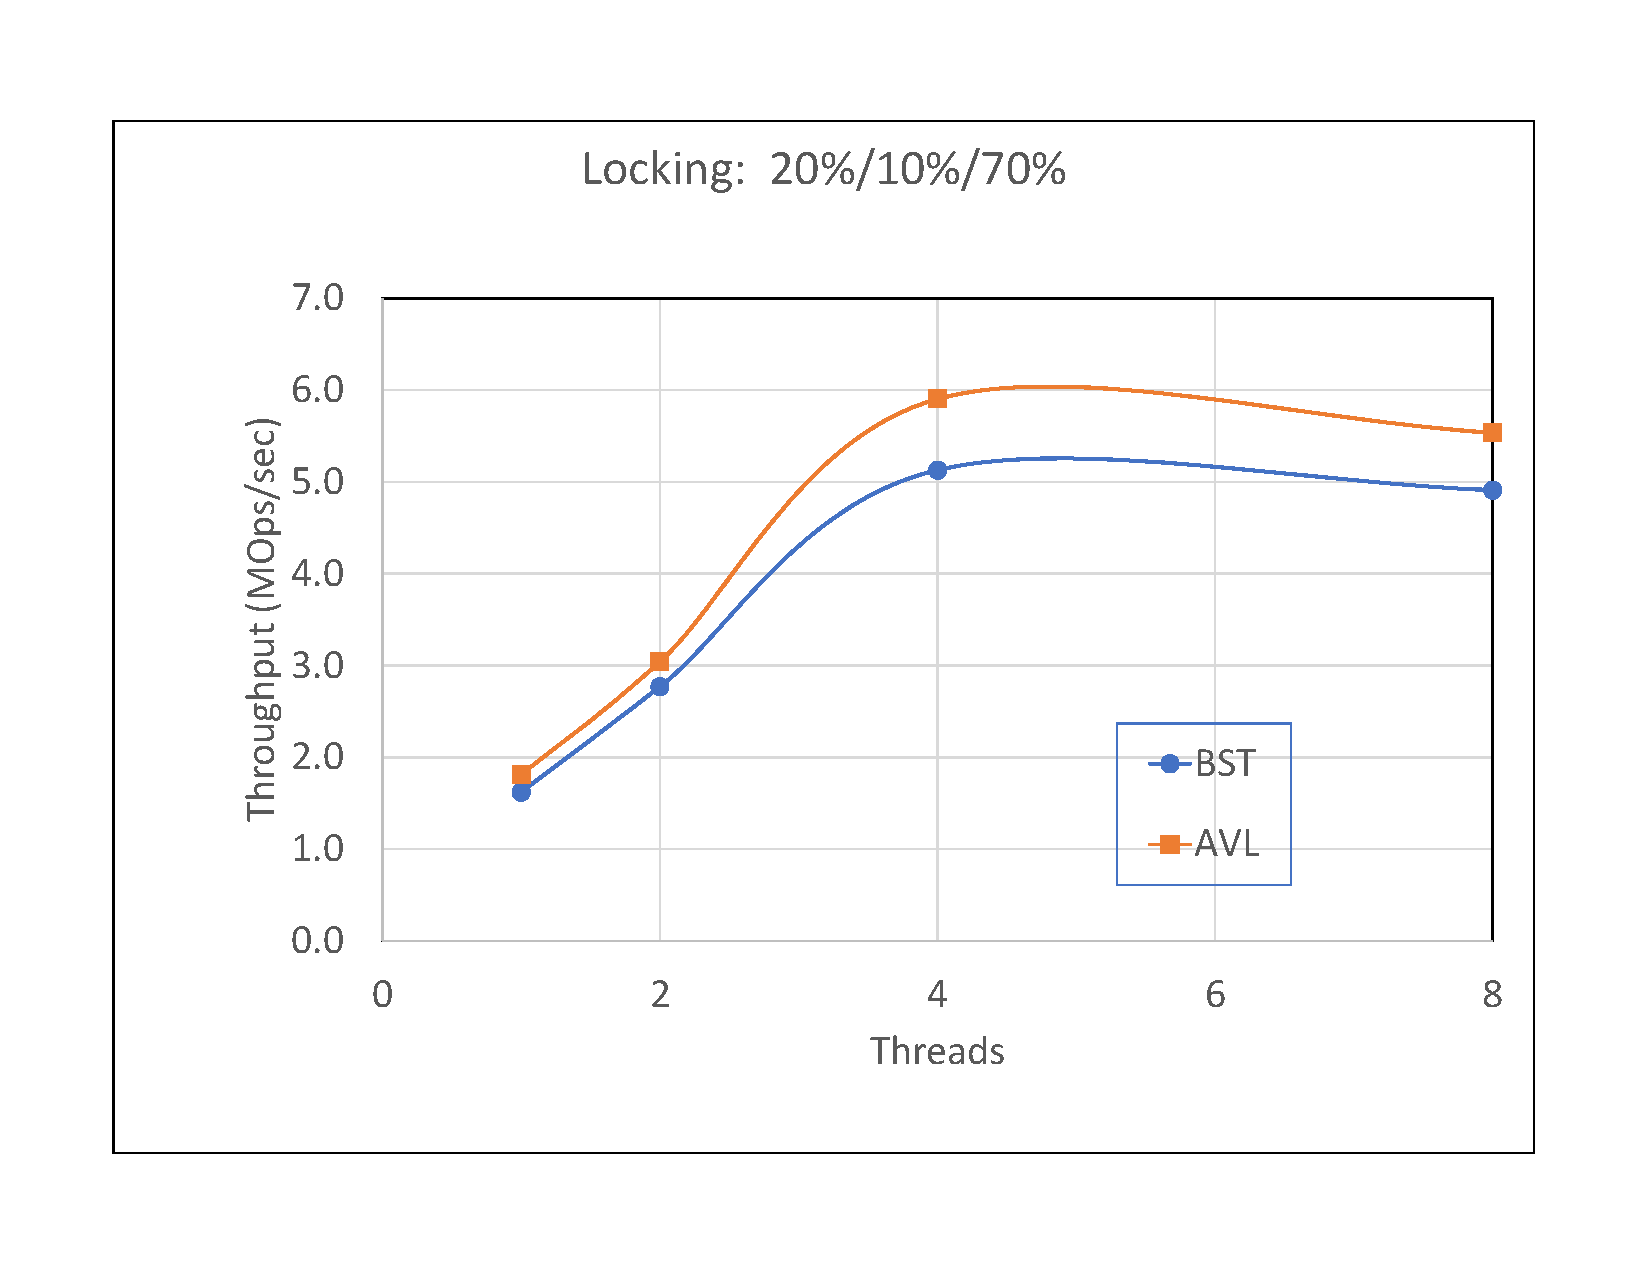
\includegraphics[width =.3\linewidth]{figures/conc-20-10-70}\hfill
%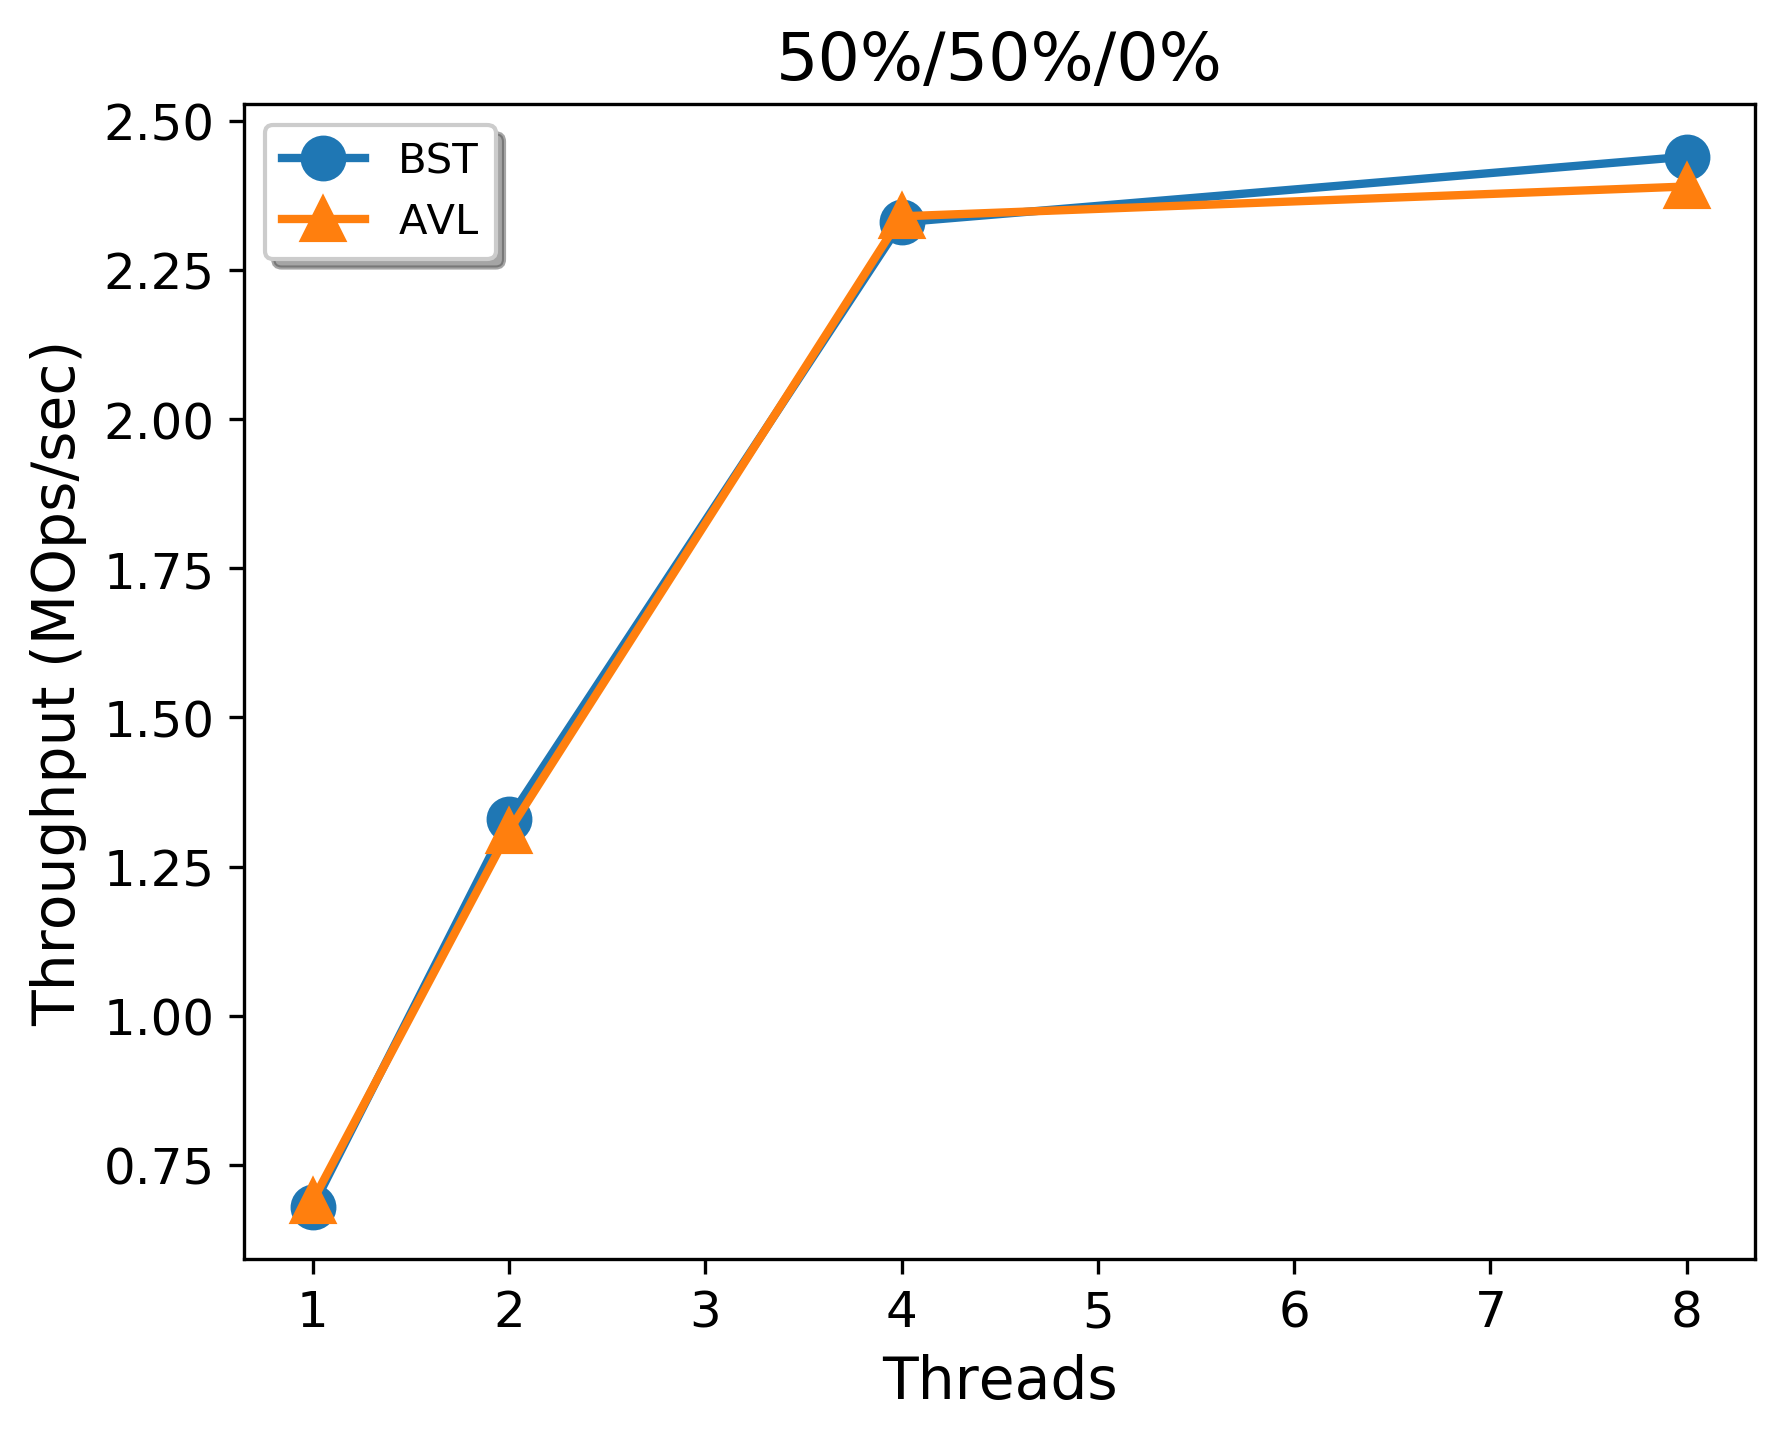
\includegraphics[width =.3\linewidth]{figures/conc-50-50-0} \\
\begin{minipage}[t][5cm][c]{\textwidth}
 \centering
 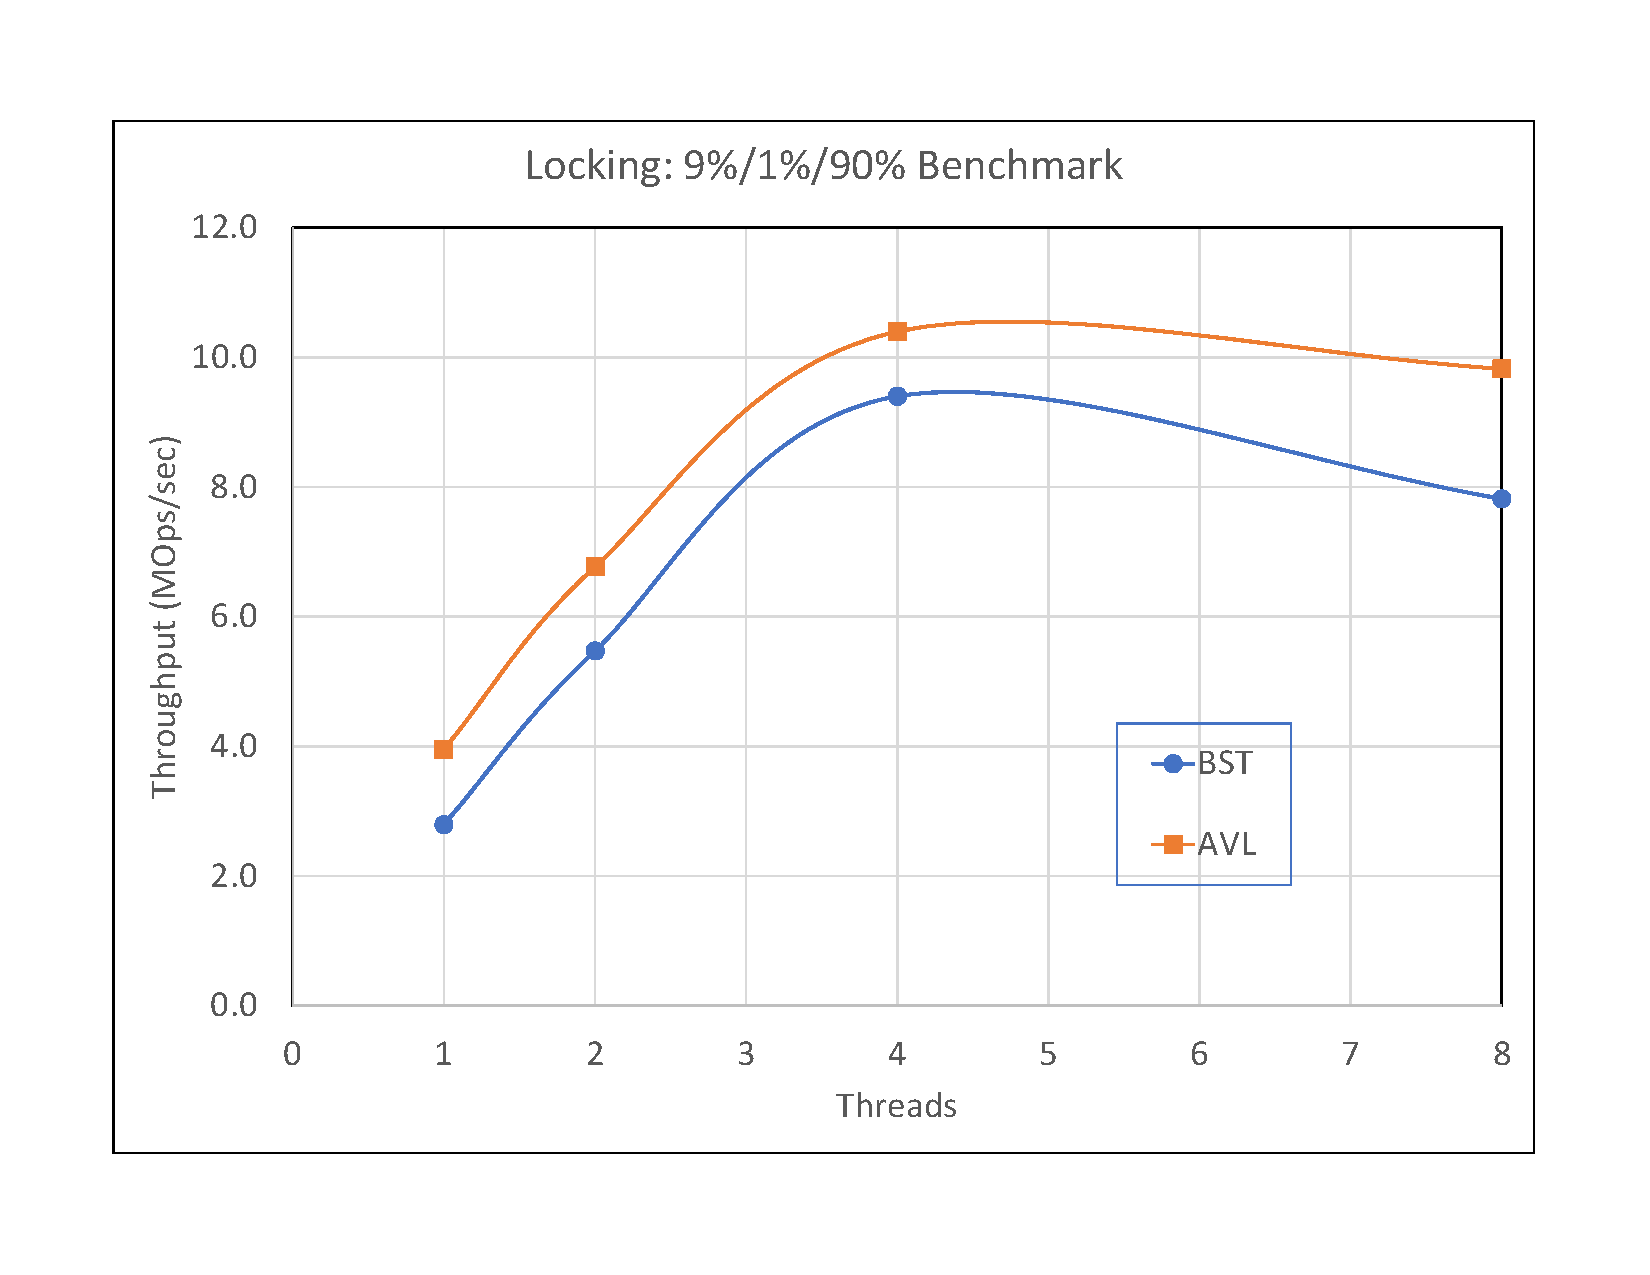
\includegraphics[width =.3\linewidth]{figures/conc-9-1-90}
 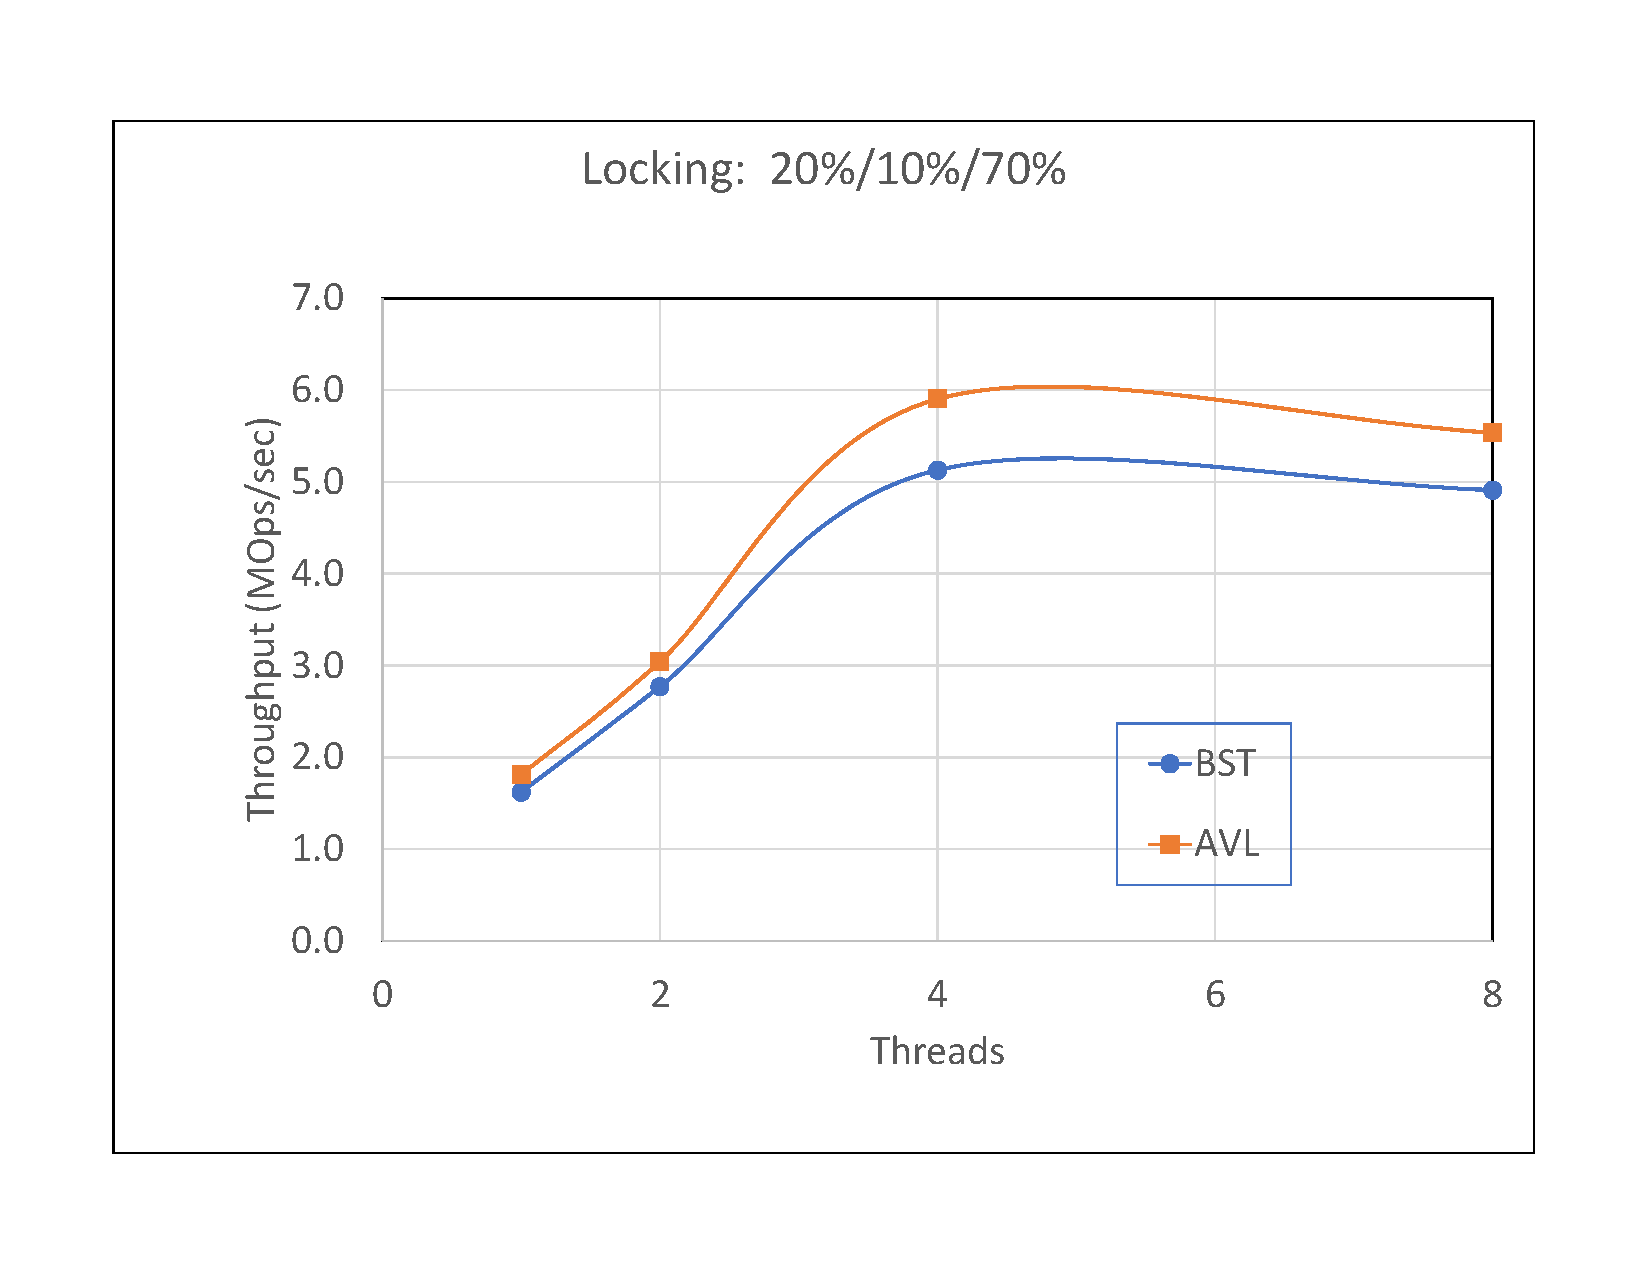
\includegraphics[width =.3\linewidth]{figures/conc-20-10-70}
 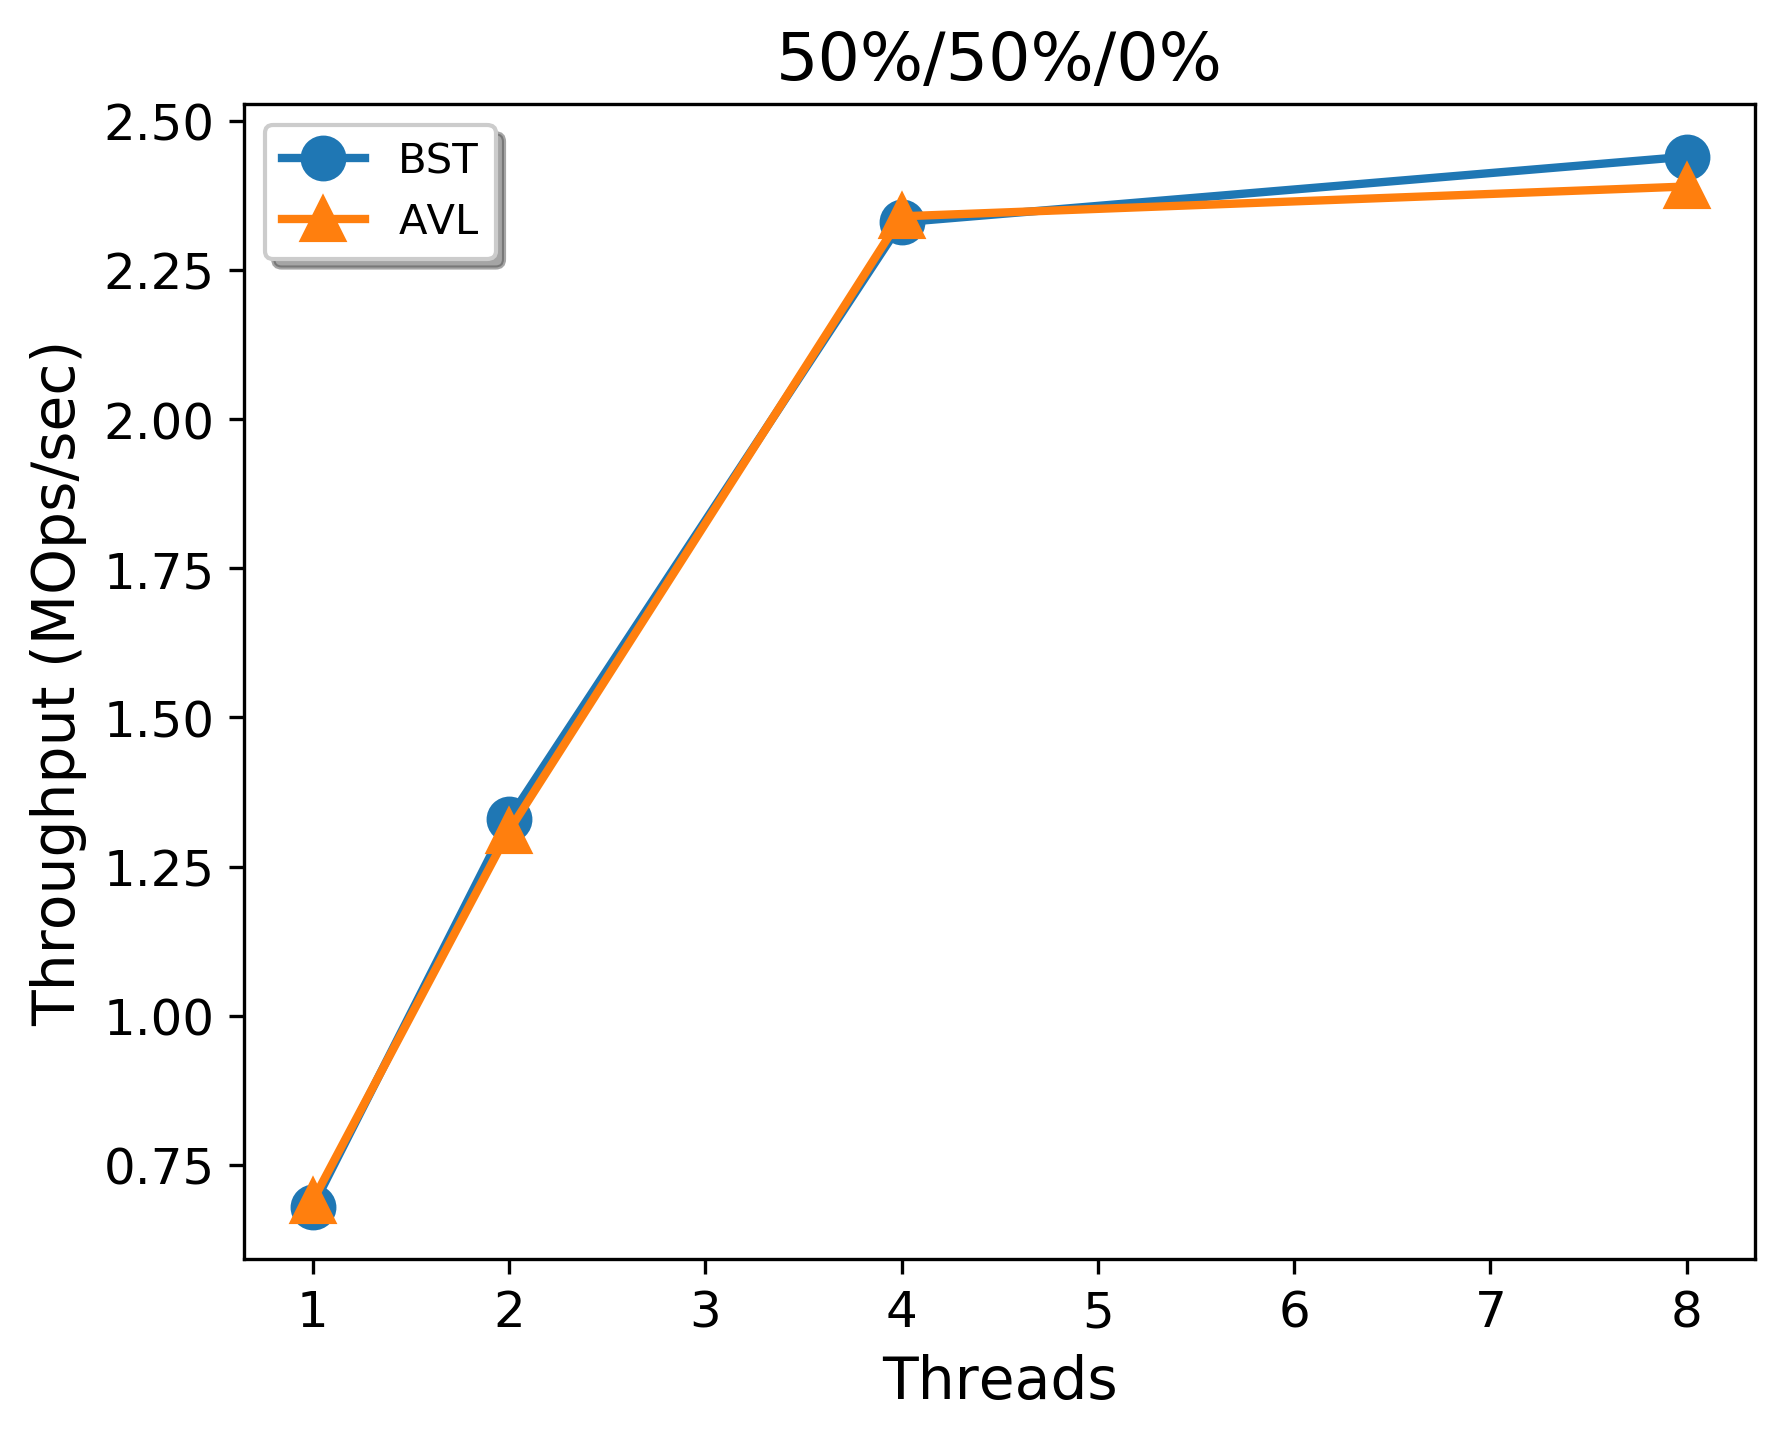
\includegraphics[width =.3\linewidth]{figures/conc-50-50-0} \\
 \captionof{figure}{Concurrent Data Structure Tests}
 \label{fig:fig1}
\end{minipage}%

\begin{minipage}[c][5cm][c]{\textwidth}
 \centering
 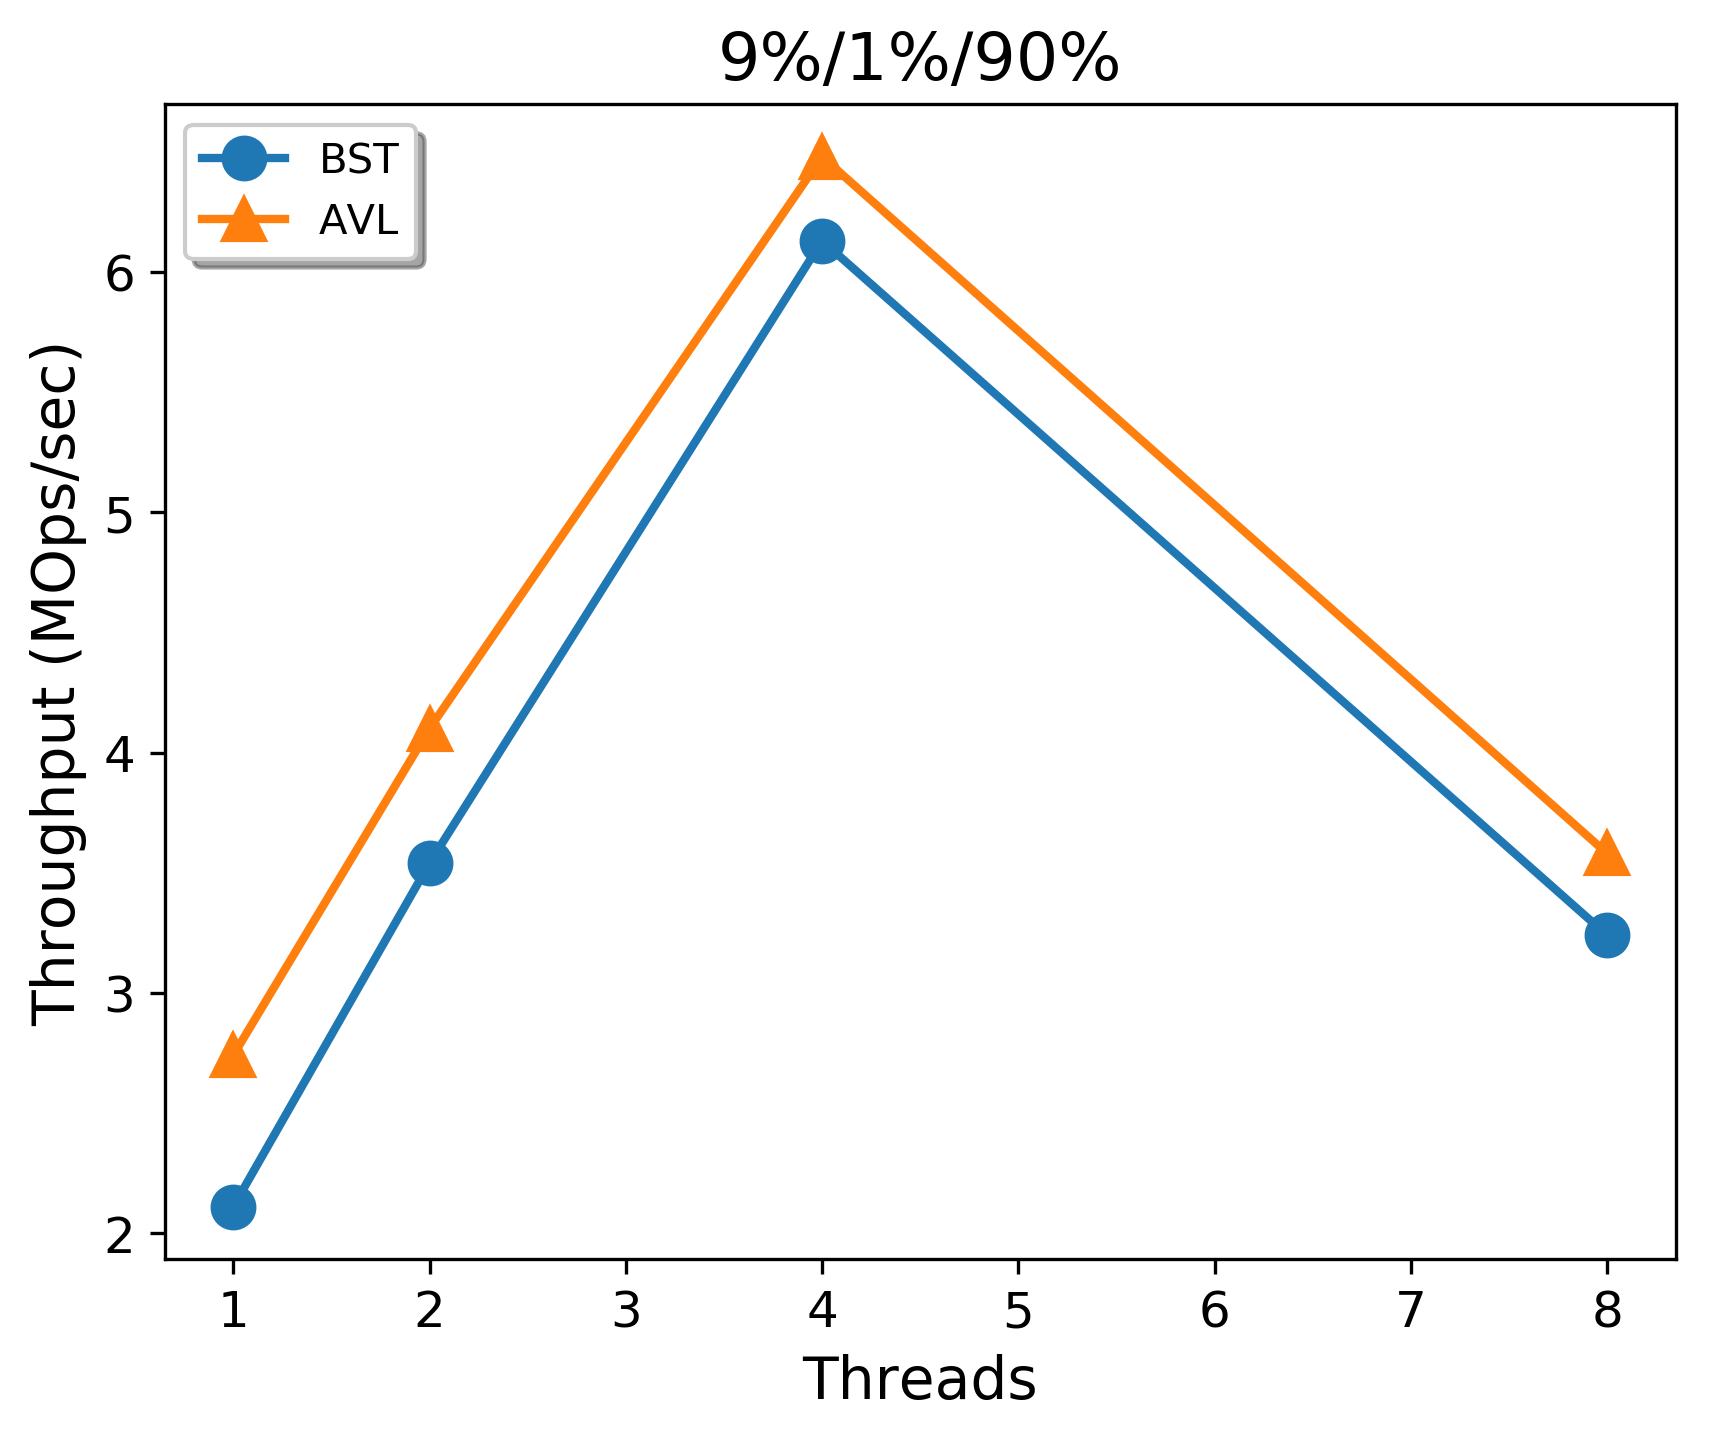
\includegraphics[width =.3\linewidth]{figures/stm1-9-1-90}
 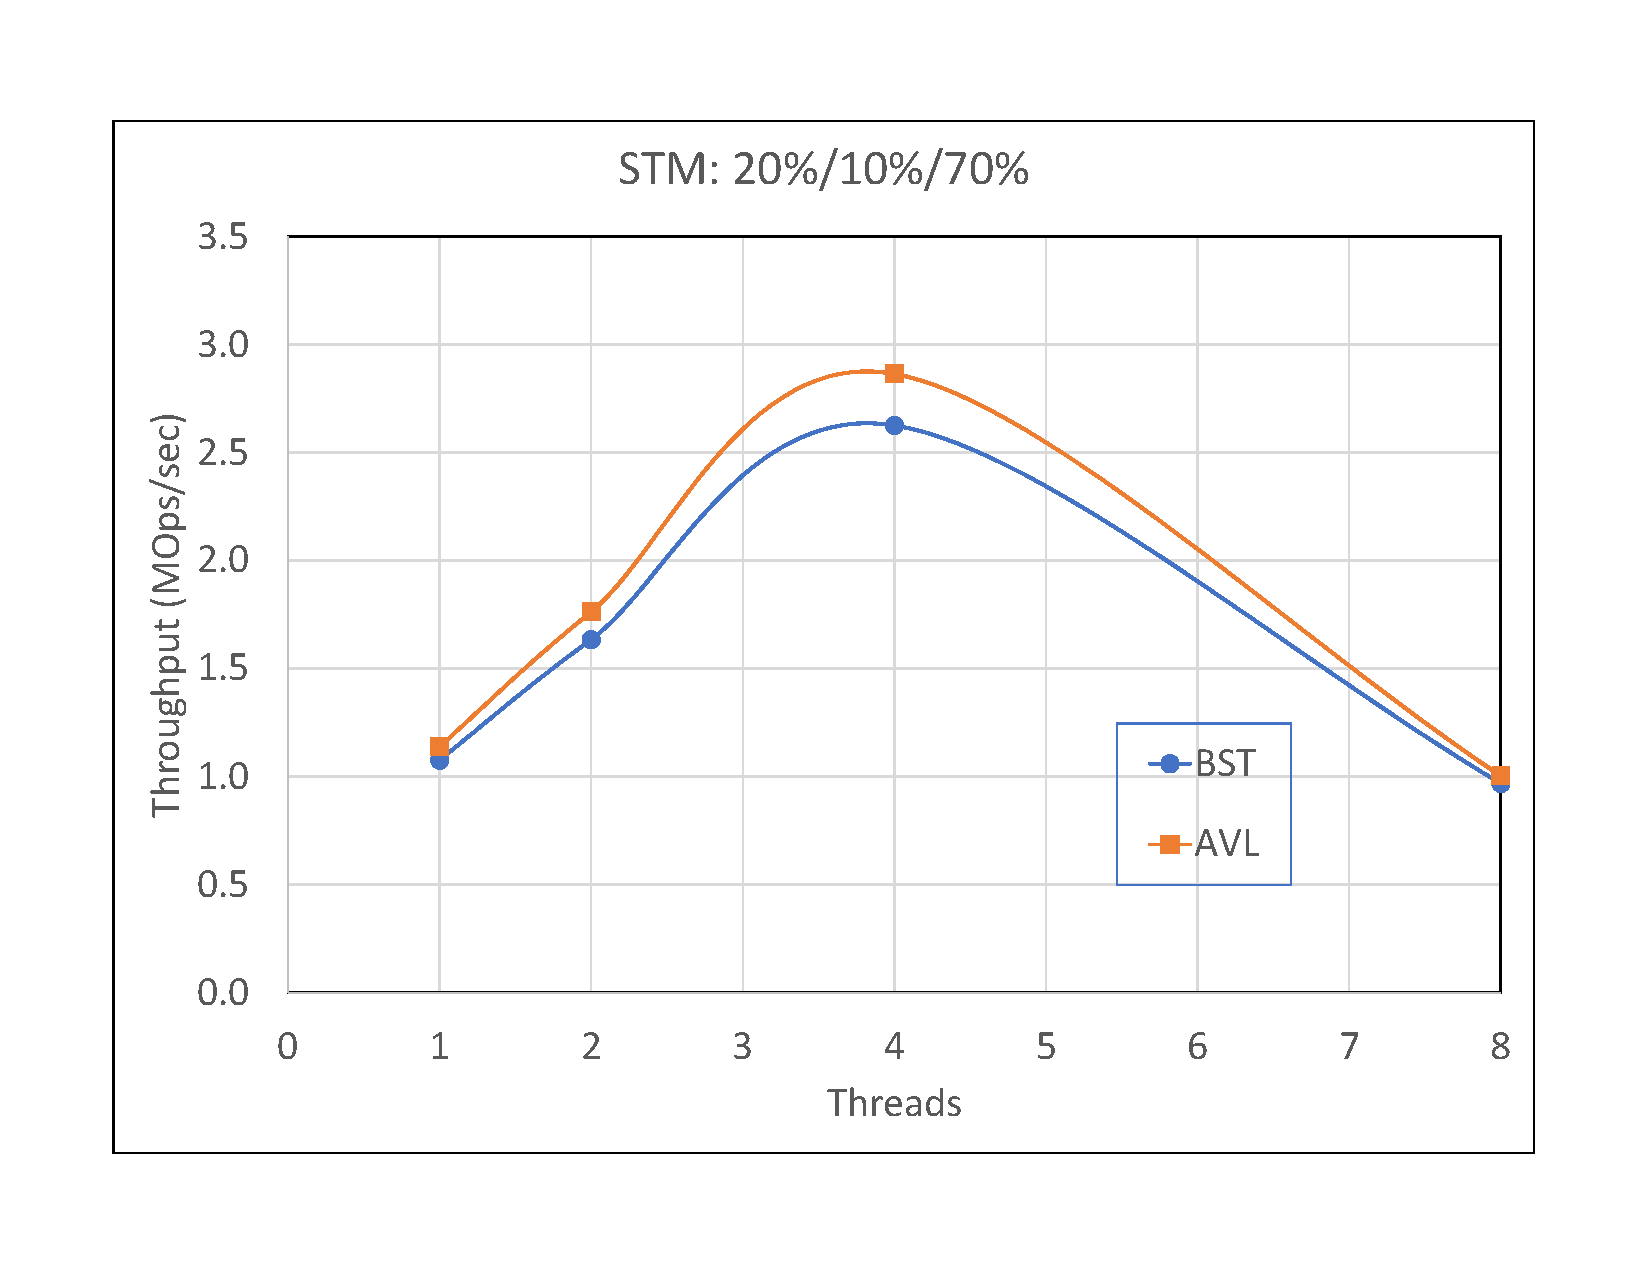
\includegraphics[width =.3\linewidth]{figures/stm1-20-10-70}
 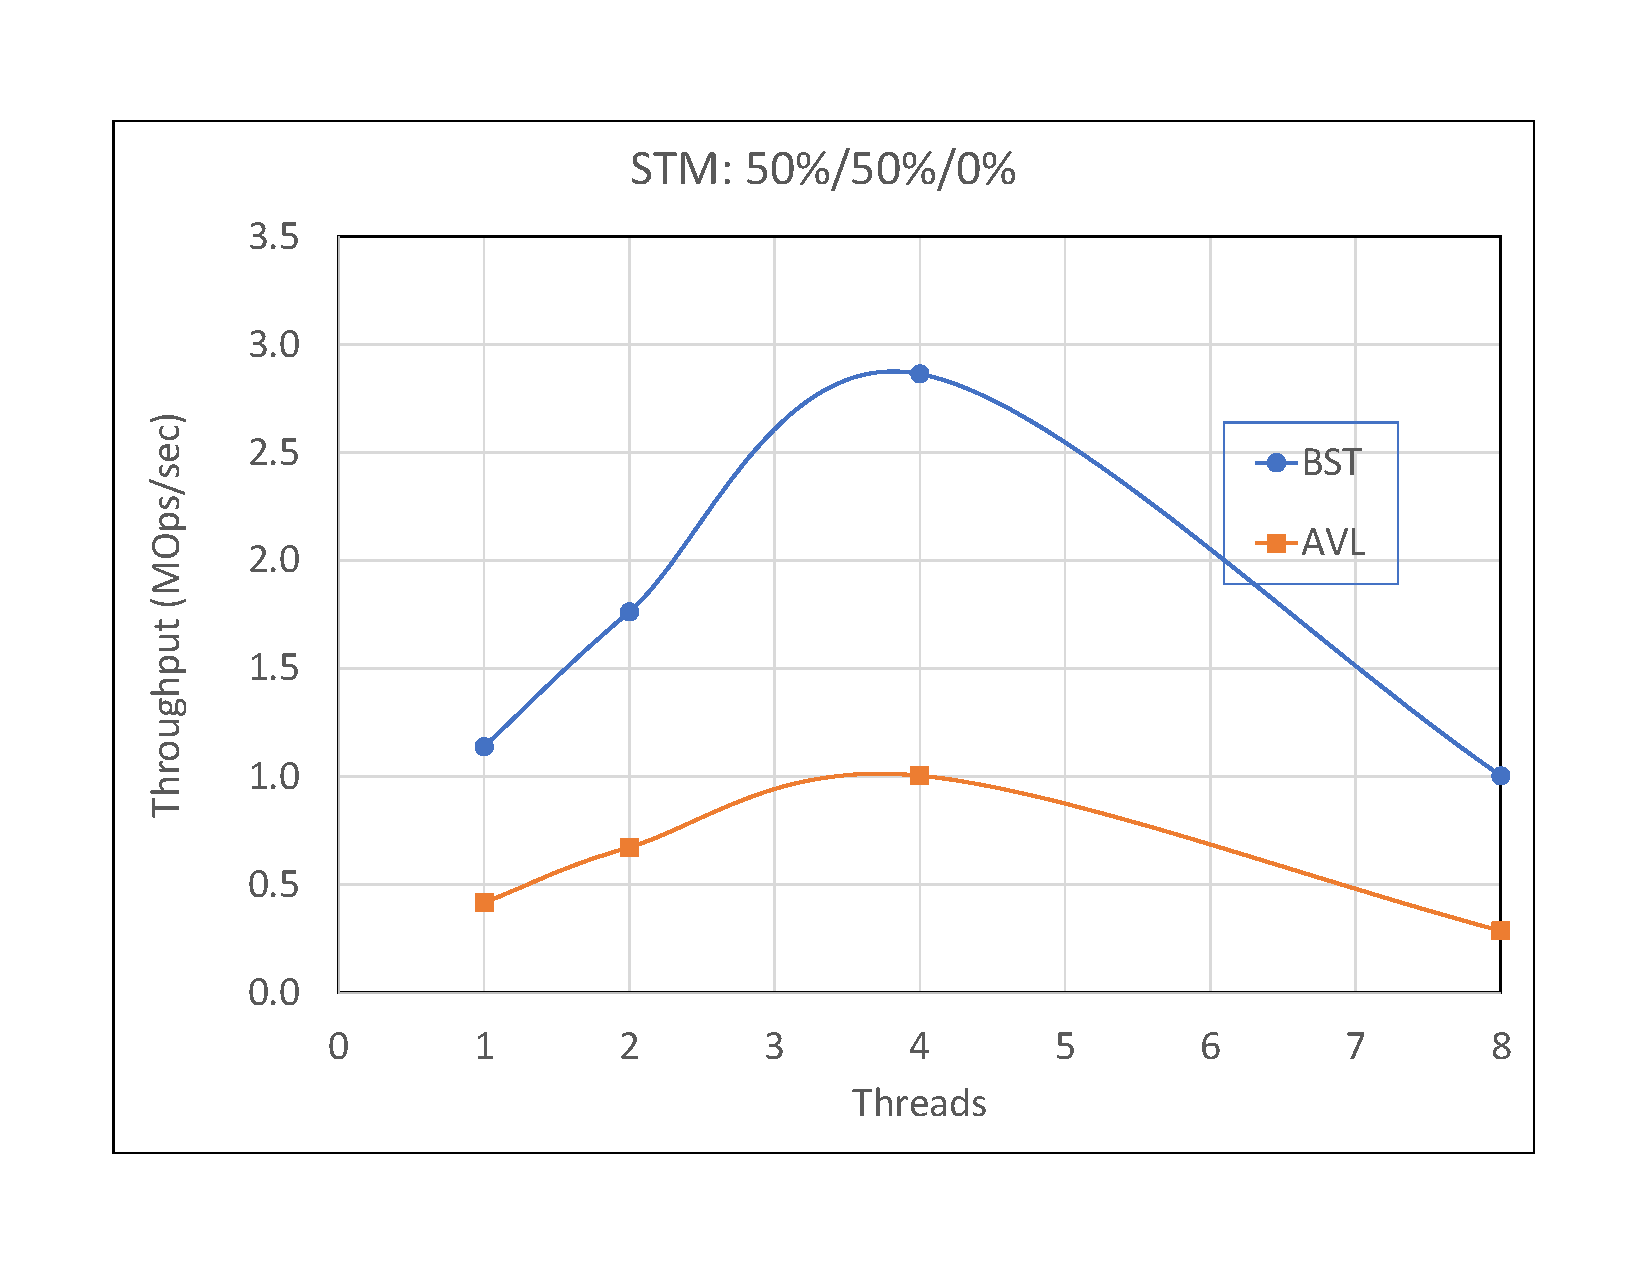
\includegraphics[width =.3\linewidth]{figures/stm1-50-50-0}
 \label{fig:fig2}
\end{minipage}%

\begin{minipage}[b][5cm][c]{\textwidth}
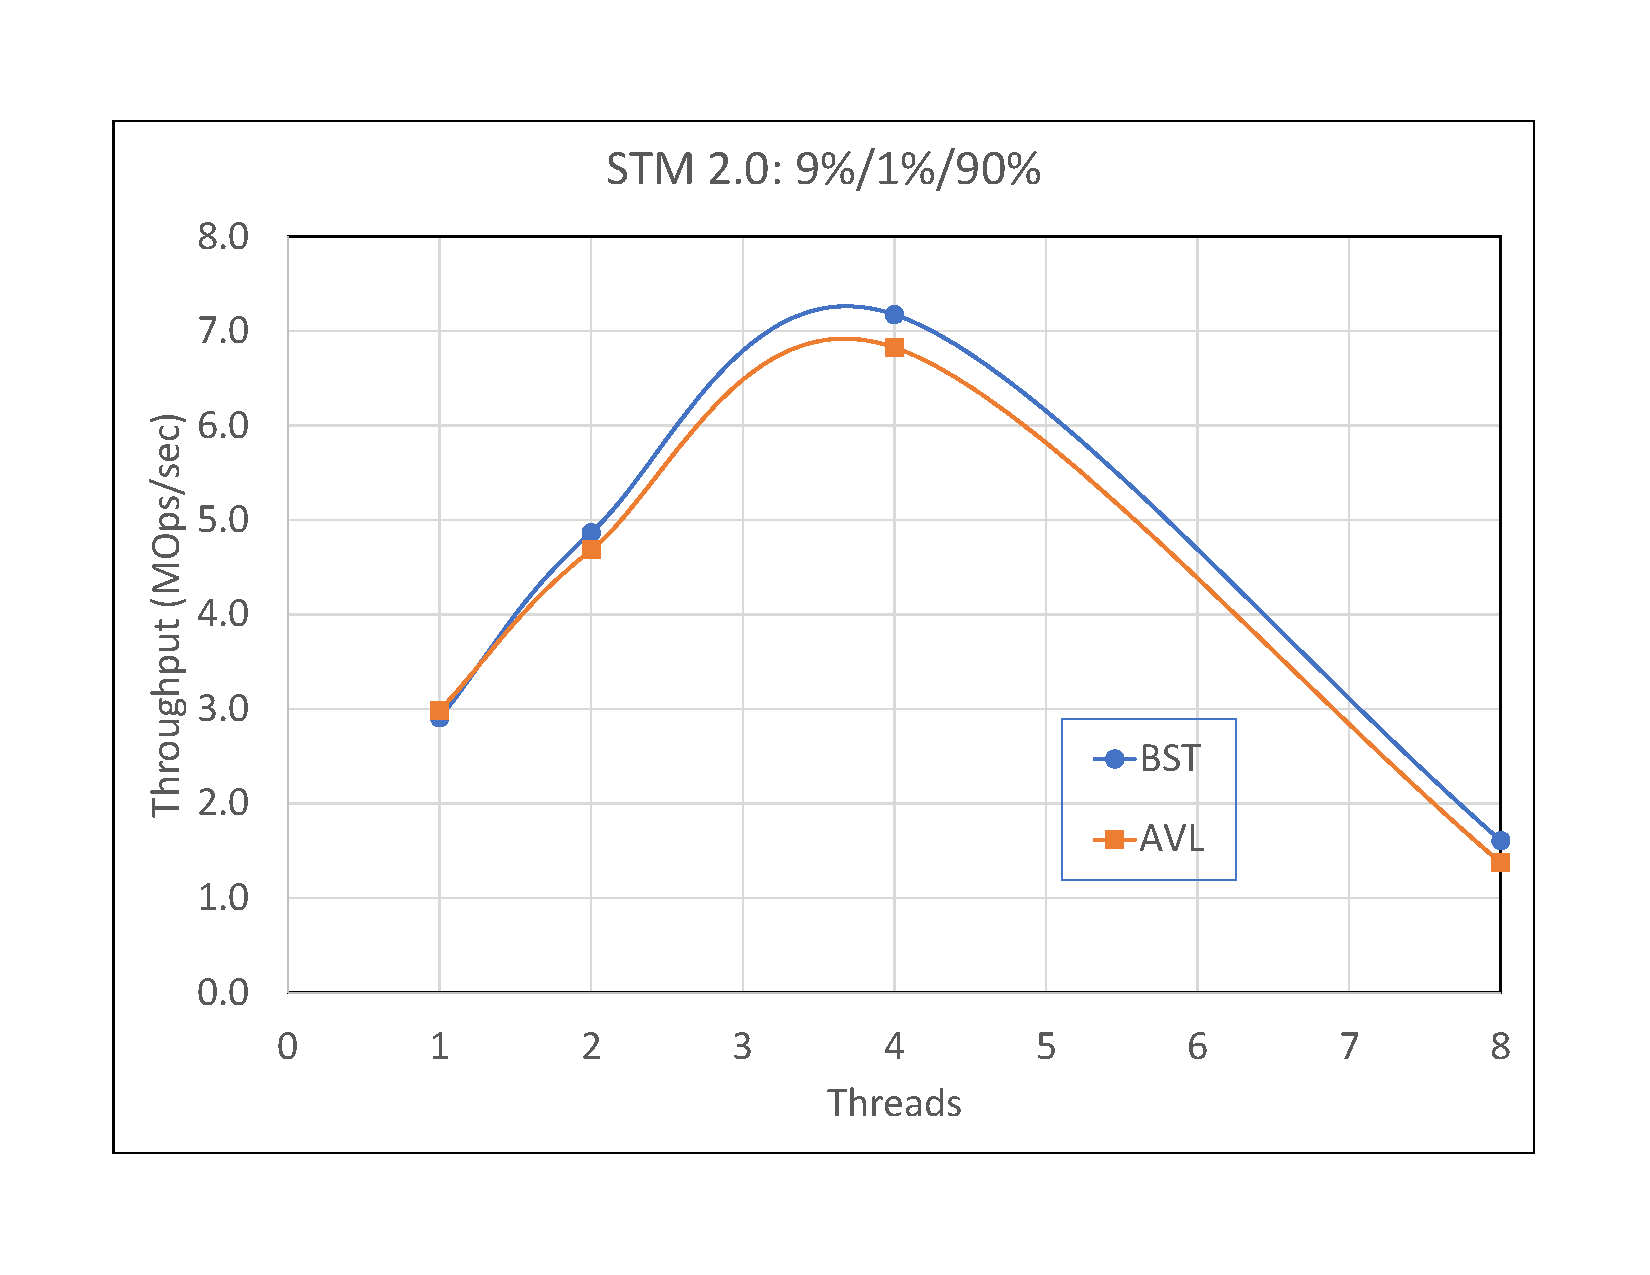
\includegraphics[width =.5\textwidth]{figures/stm2-9-1-90}
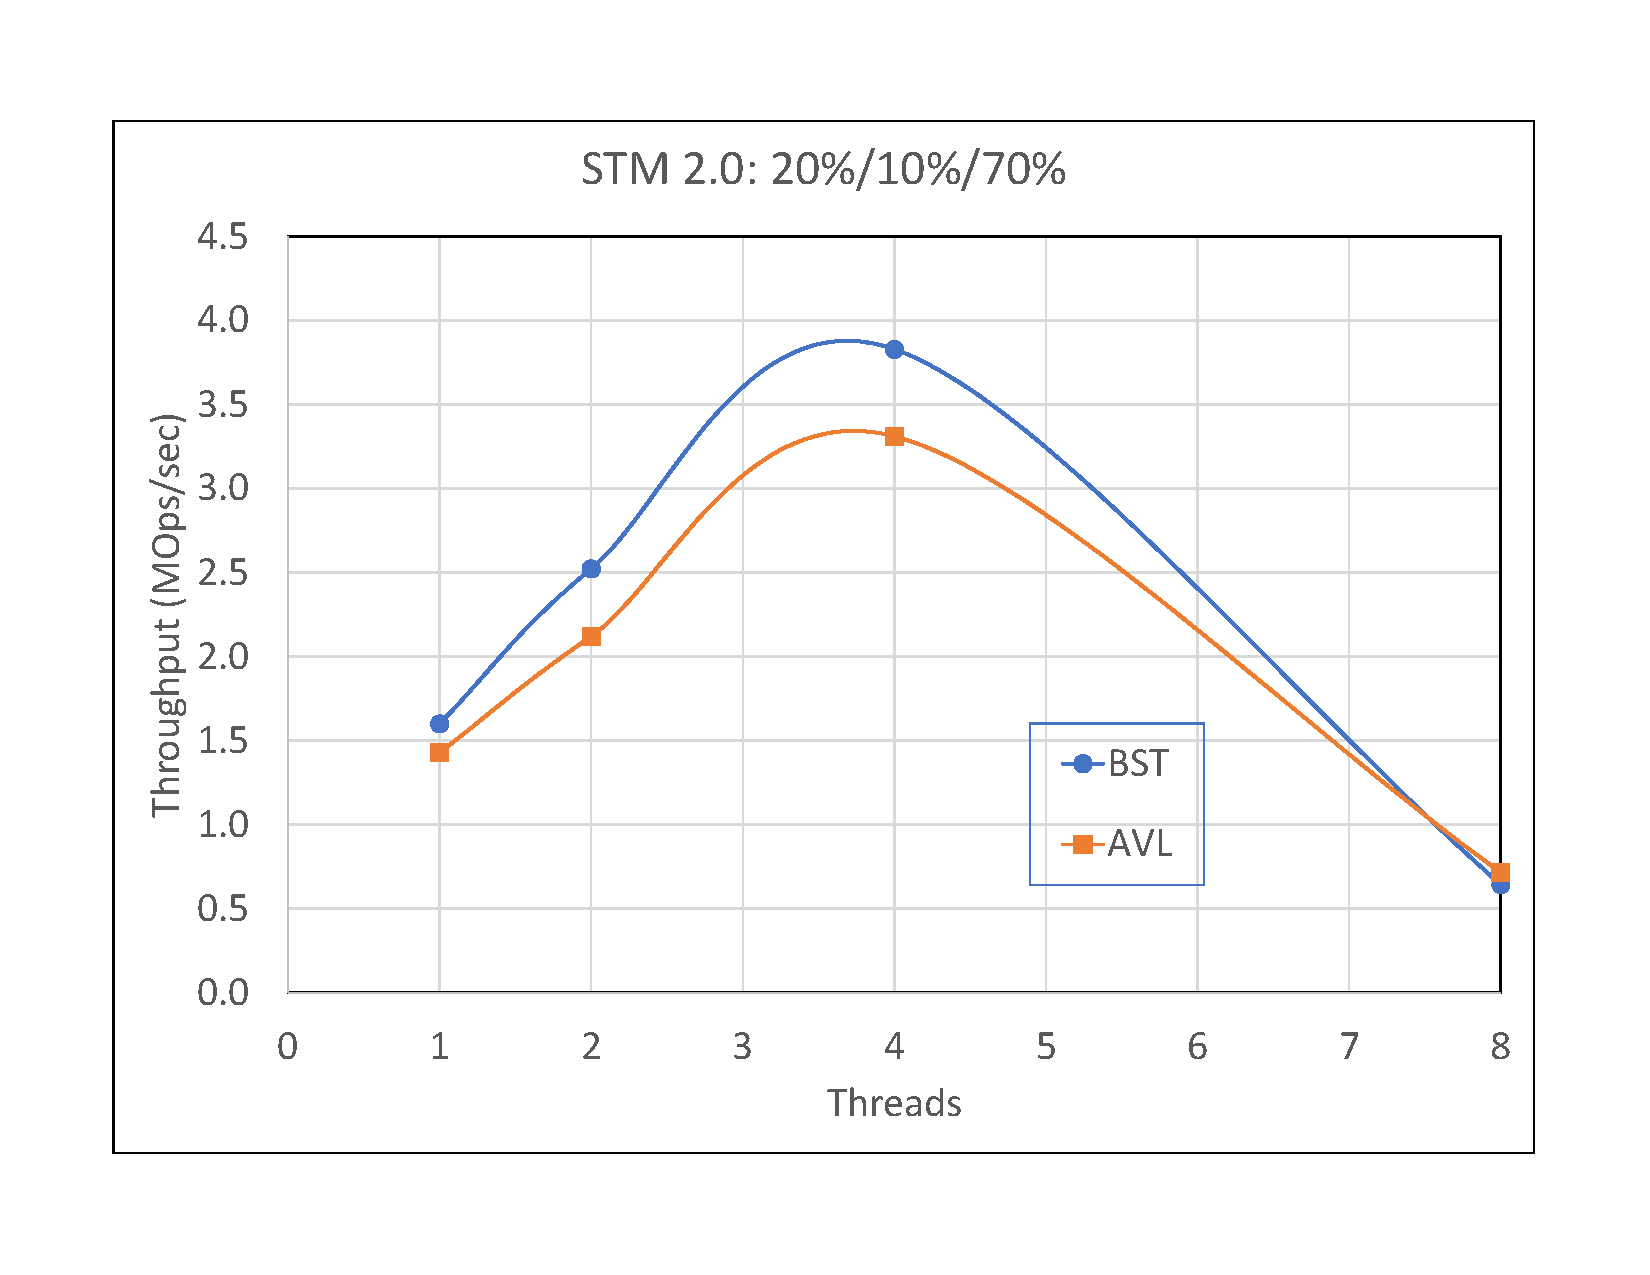
\includegraphics[width =.5\textwidth]{figures/stm2-20-10-70}
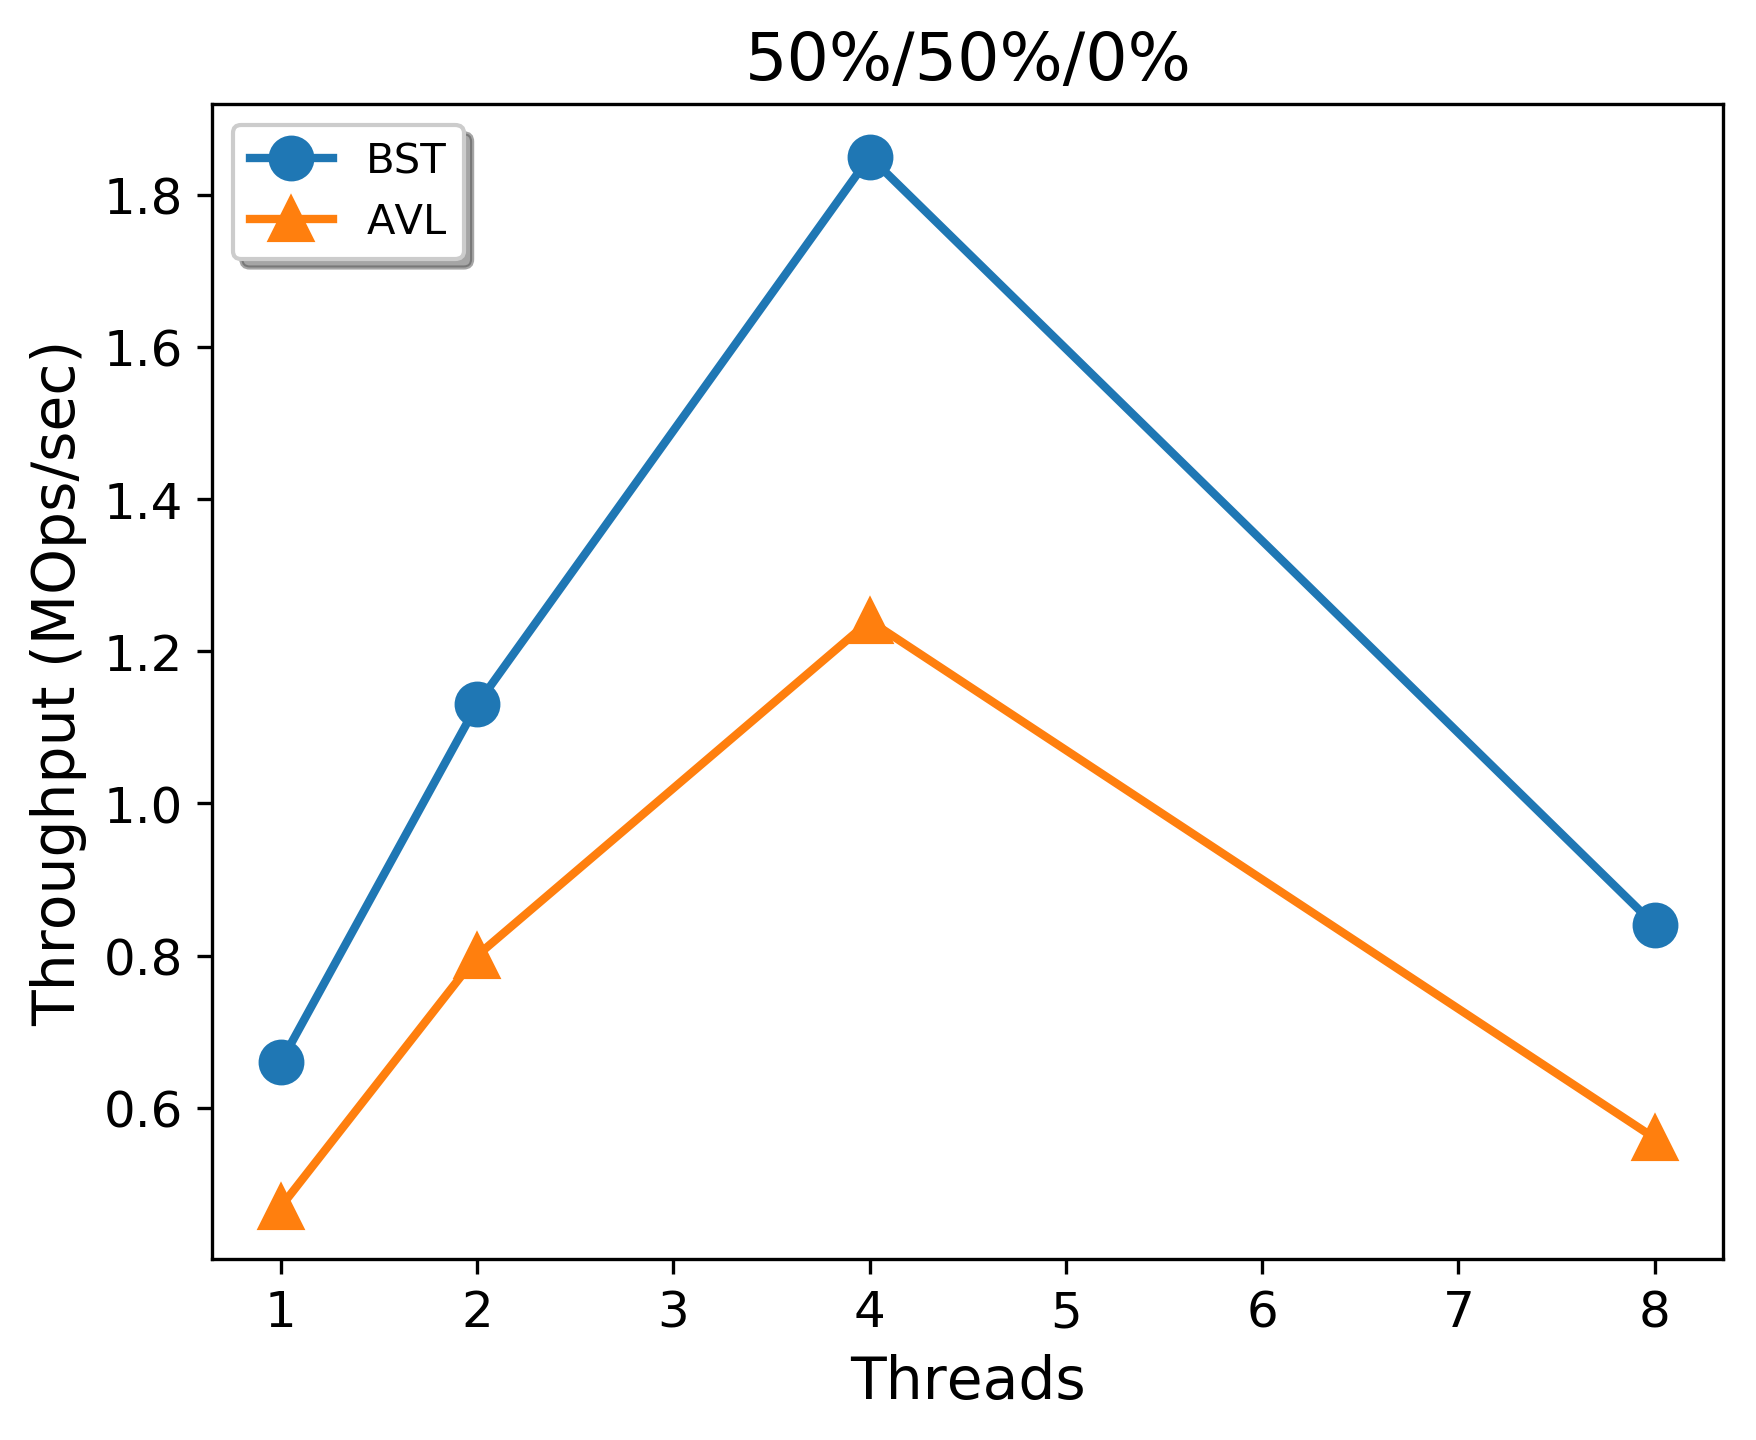
\includegraphics[width =.5\textwidth]{figures/stm2-50-50-0} \\
 \label{fig:fig1}
\end{minipage}%

\caption{adsf}
\end{figure*}%

\iffalse

\begin{figure}[H]
\begin{tabular}{c}
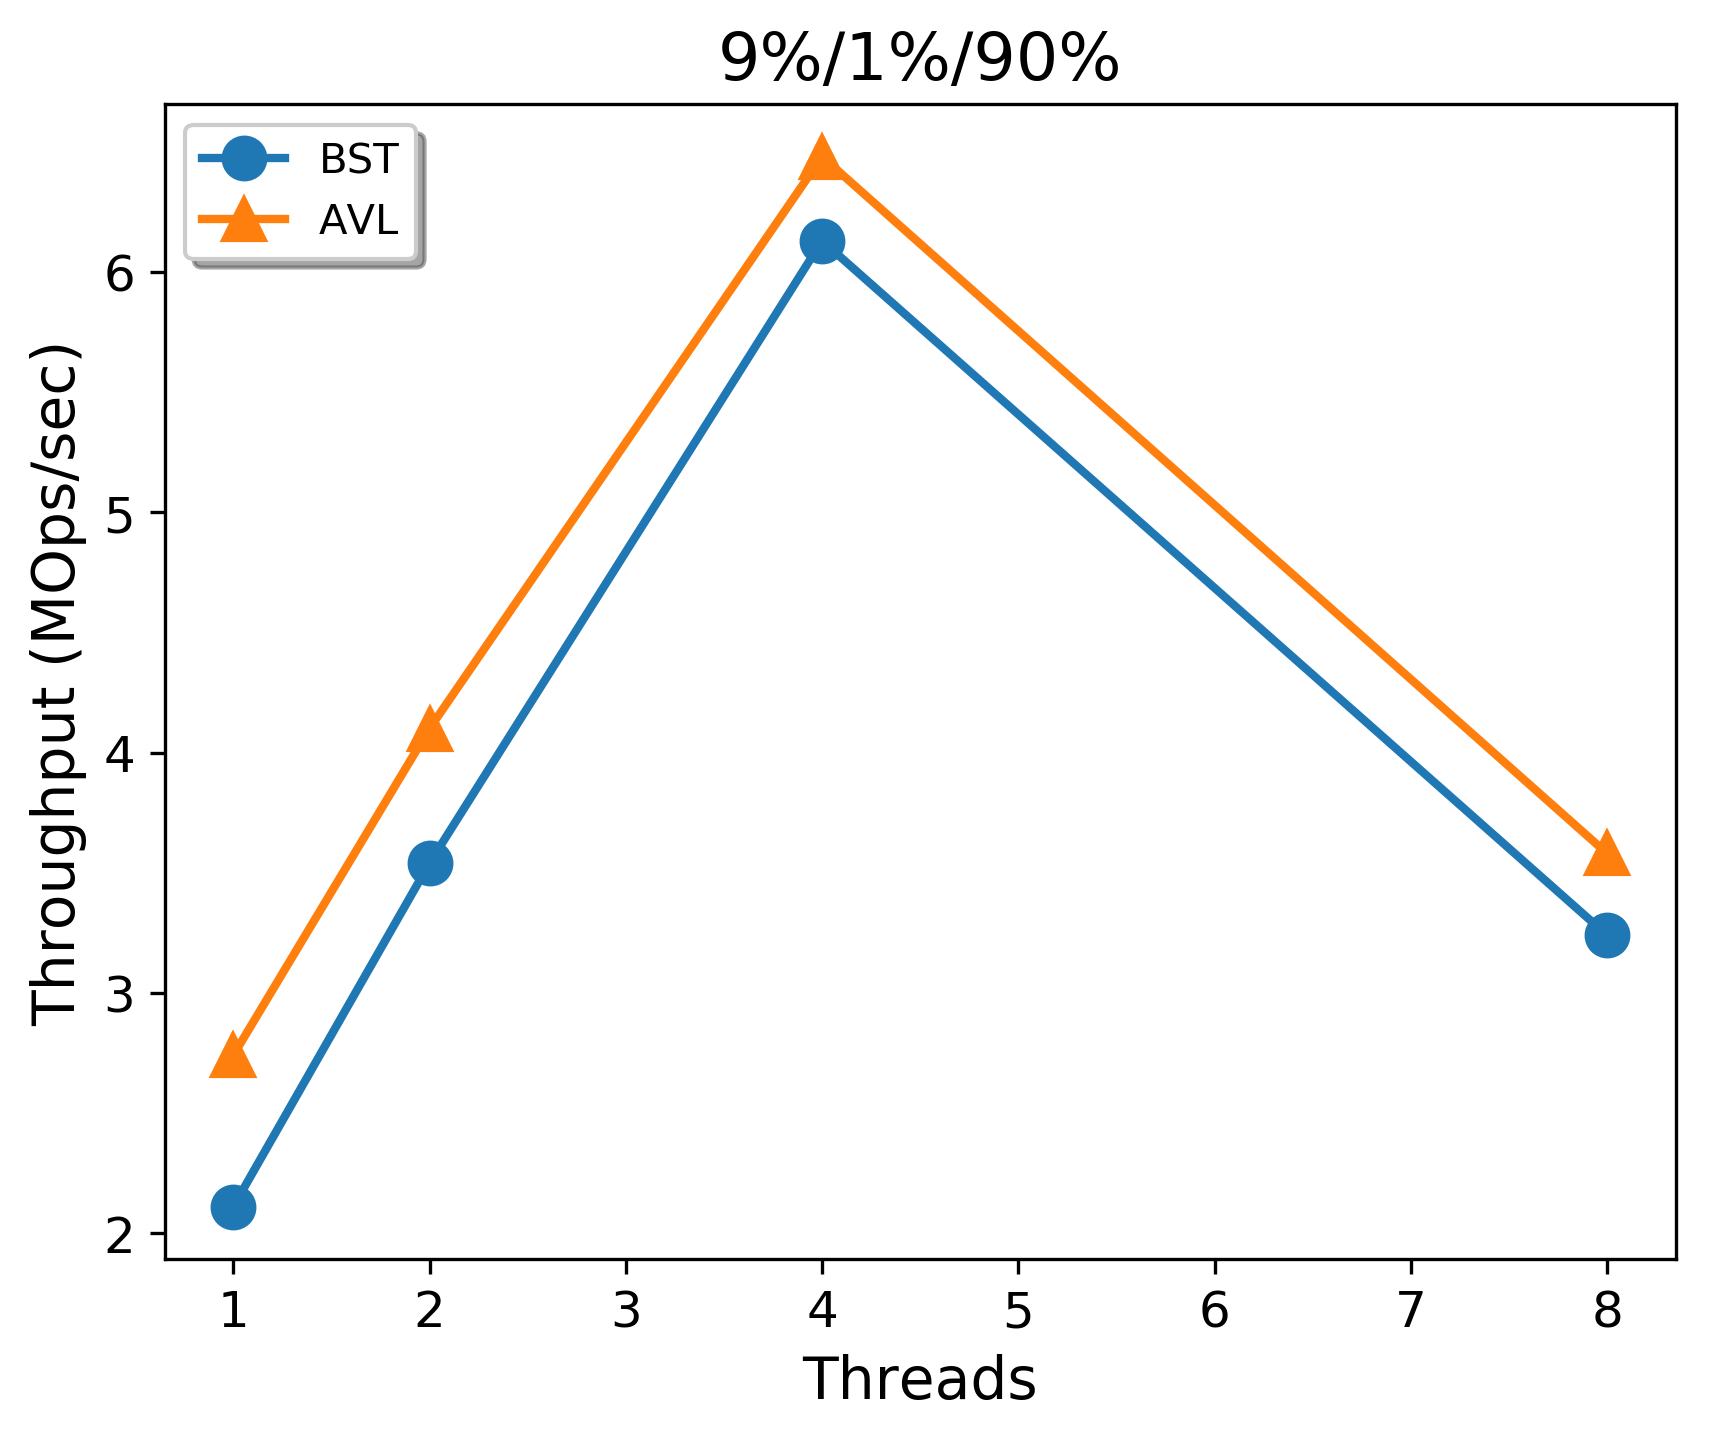
\includegraphics[width =\linewidth]{figures/stm1-9-1-90}\\
(a) \\
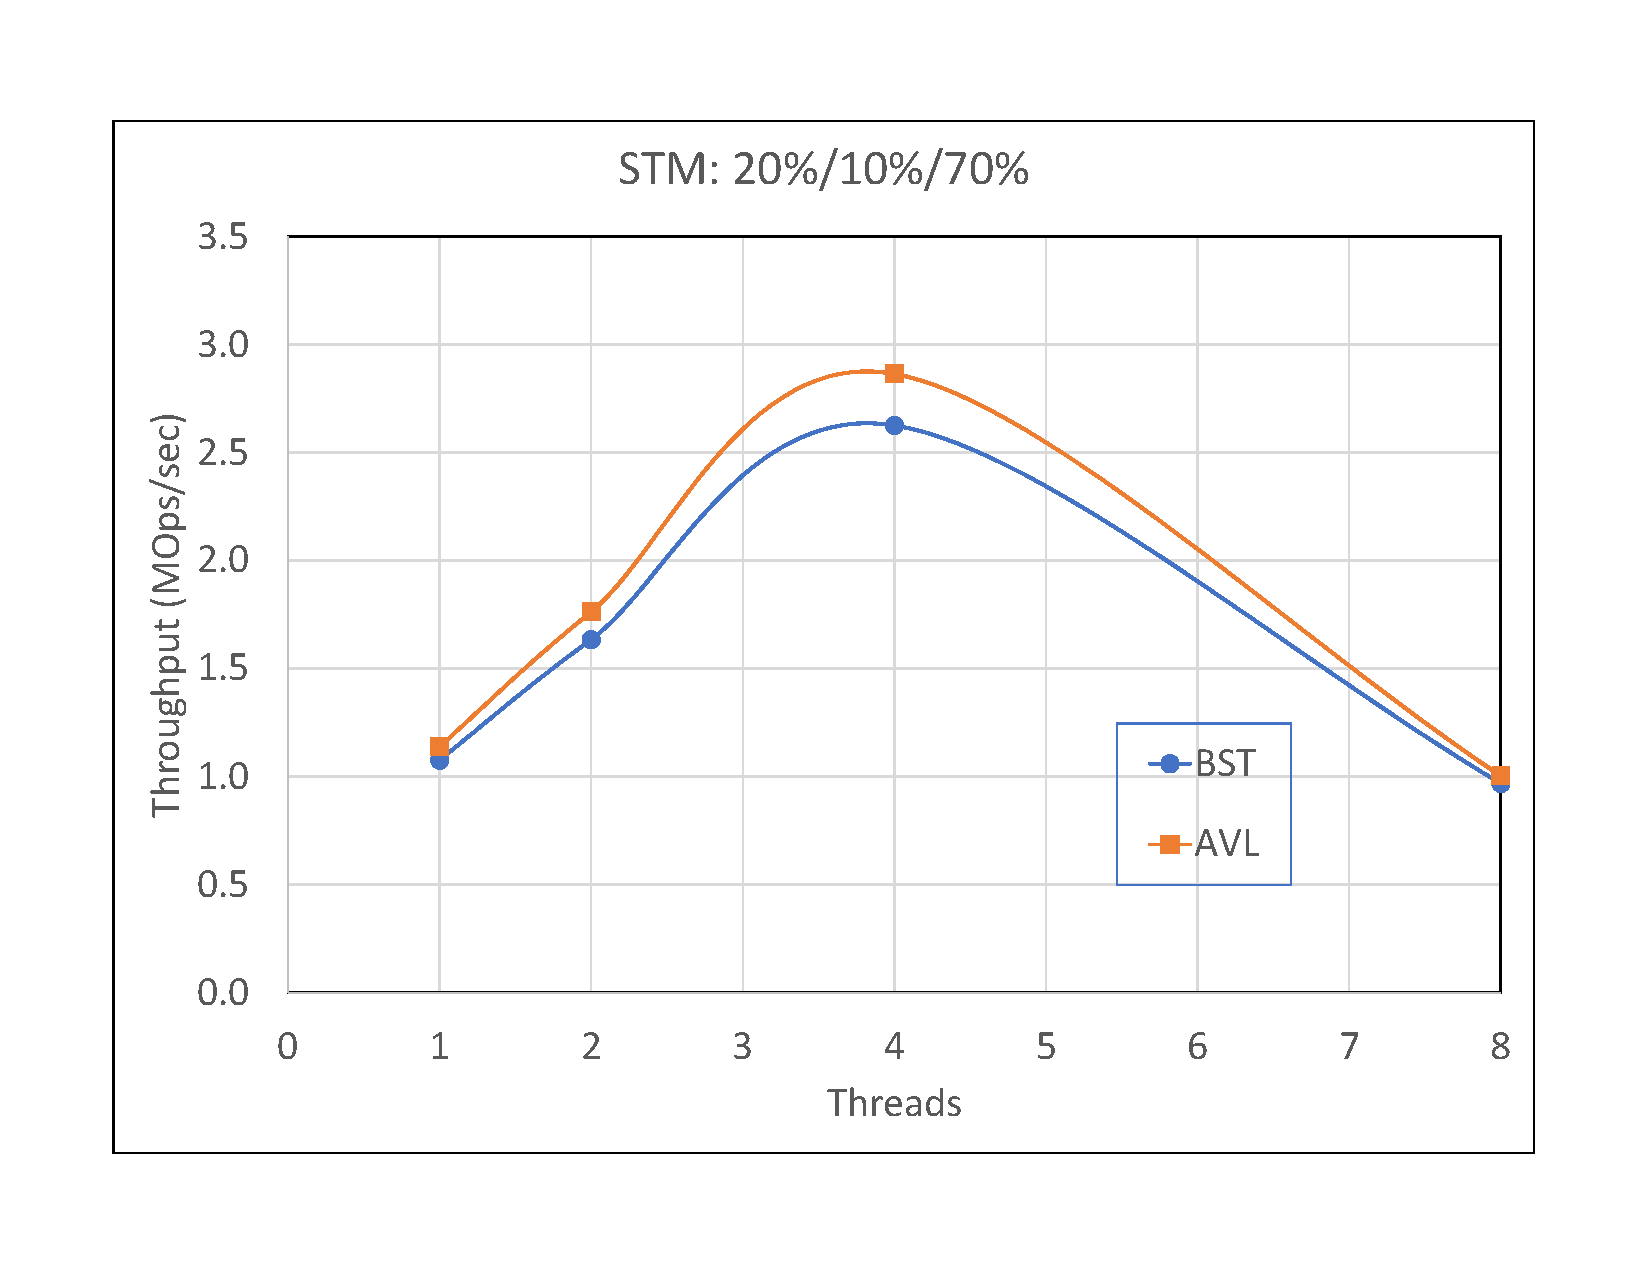
\includegraphics[width =\linewidth]{figures/stm1-20-10-70}\\
(b) \\
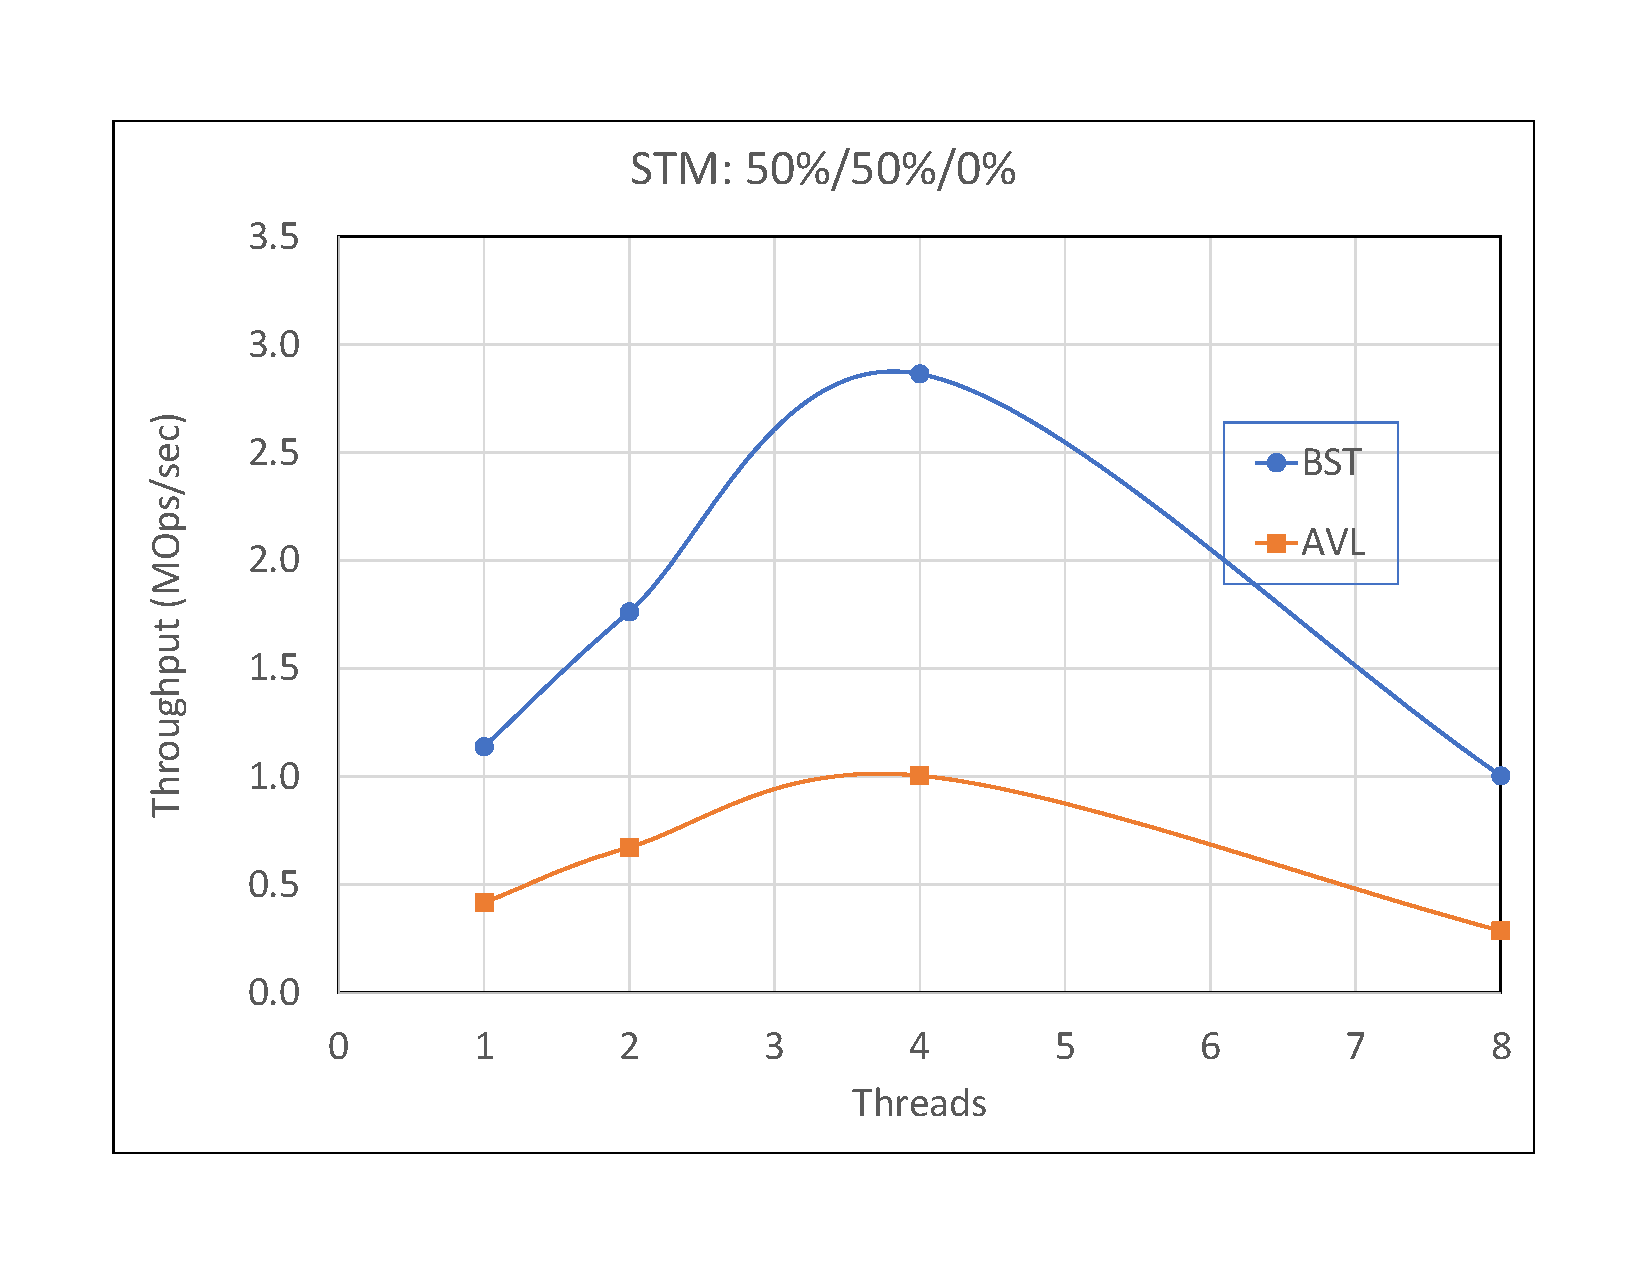
\includegraphics[width =\linewidth]{figures/stm1-50-50-0} \\
(c) 
\end{tabular}
\caption{adsf}
\end{figure}

\begin{figure*}[H]
\begin{tabular}{c}
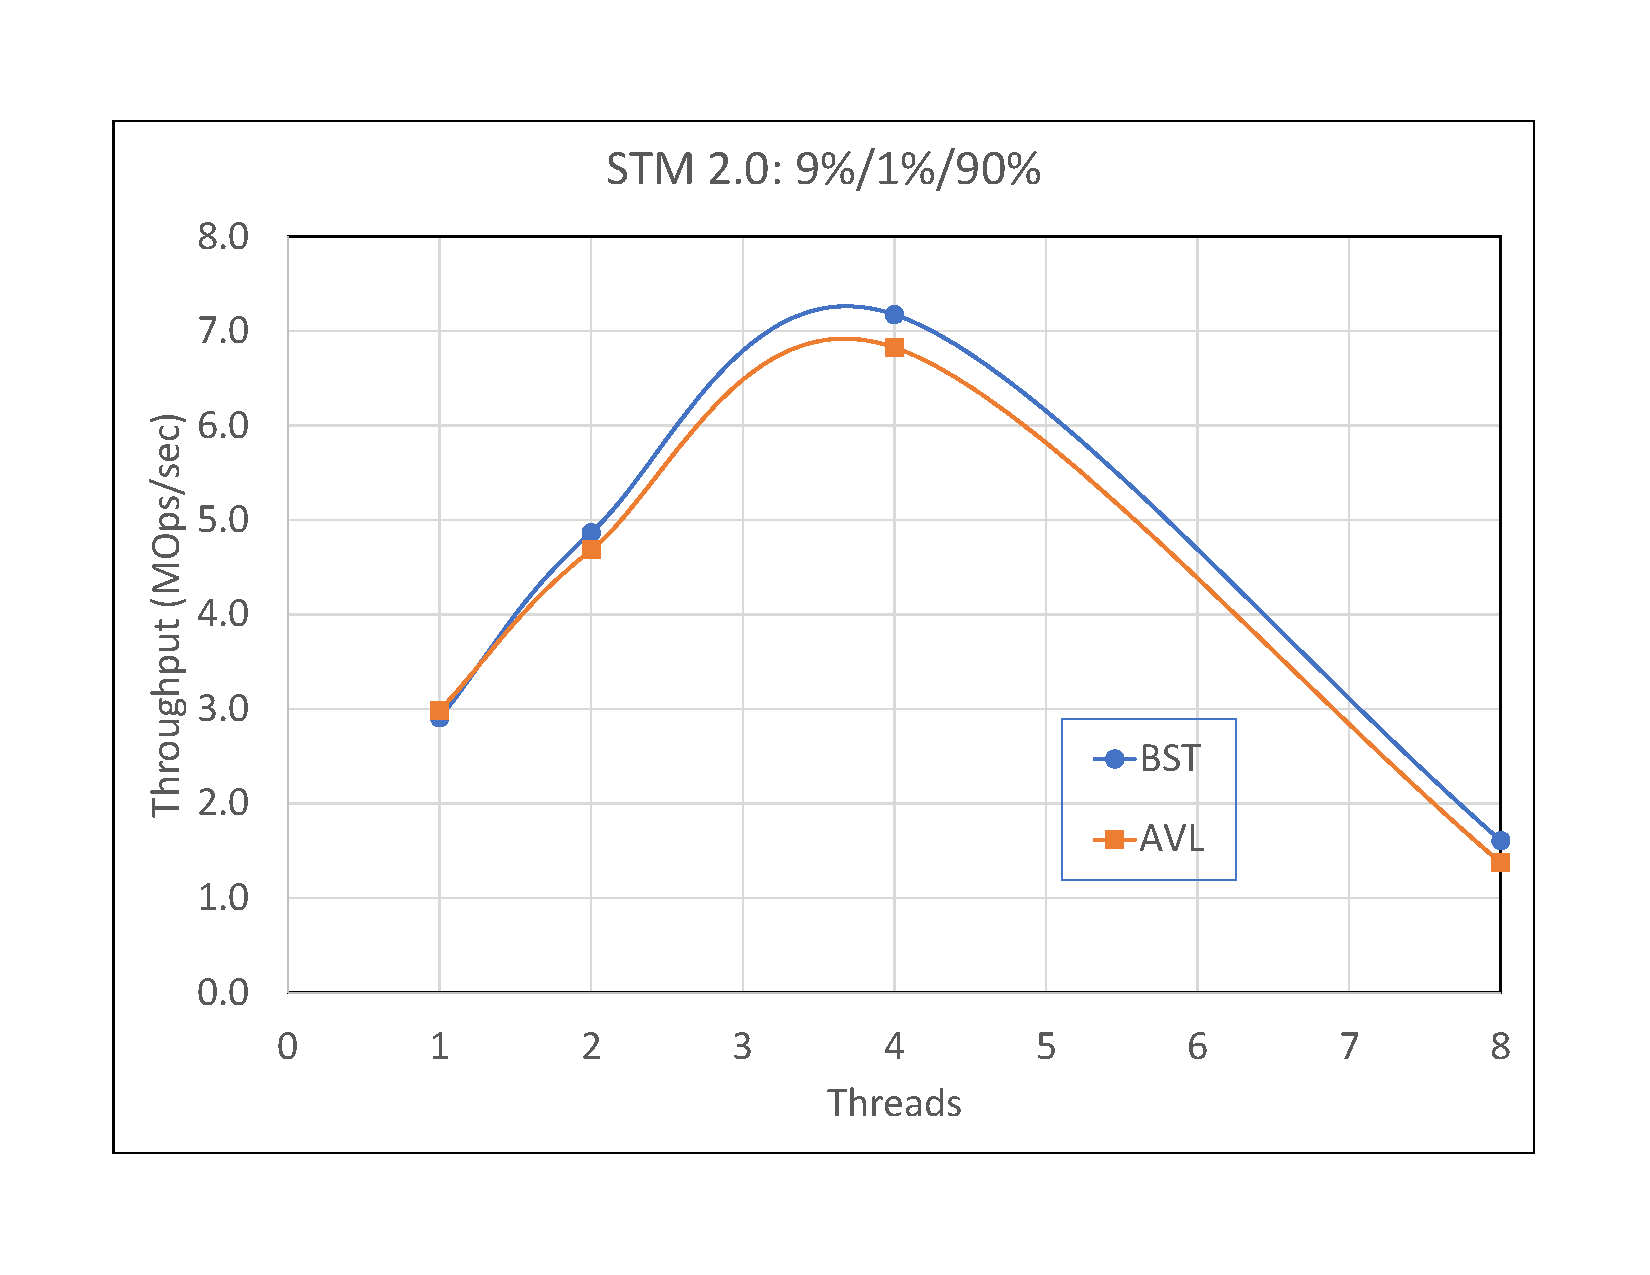
\includegraphics[width =\linewidth]{figures/stm2-9-1-90}\\
(a) \\
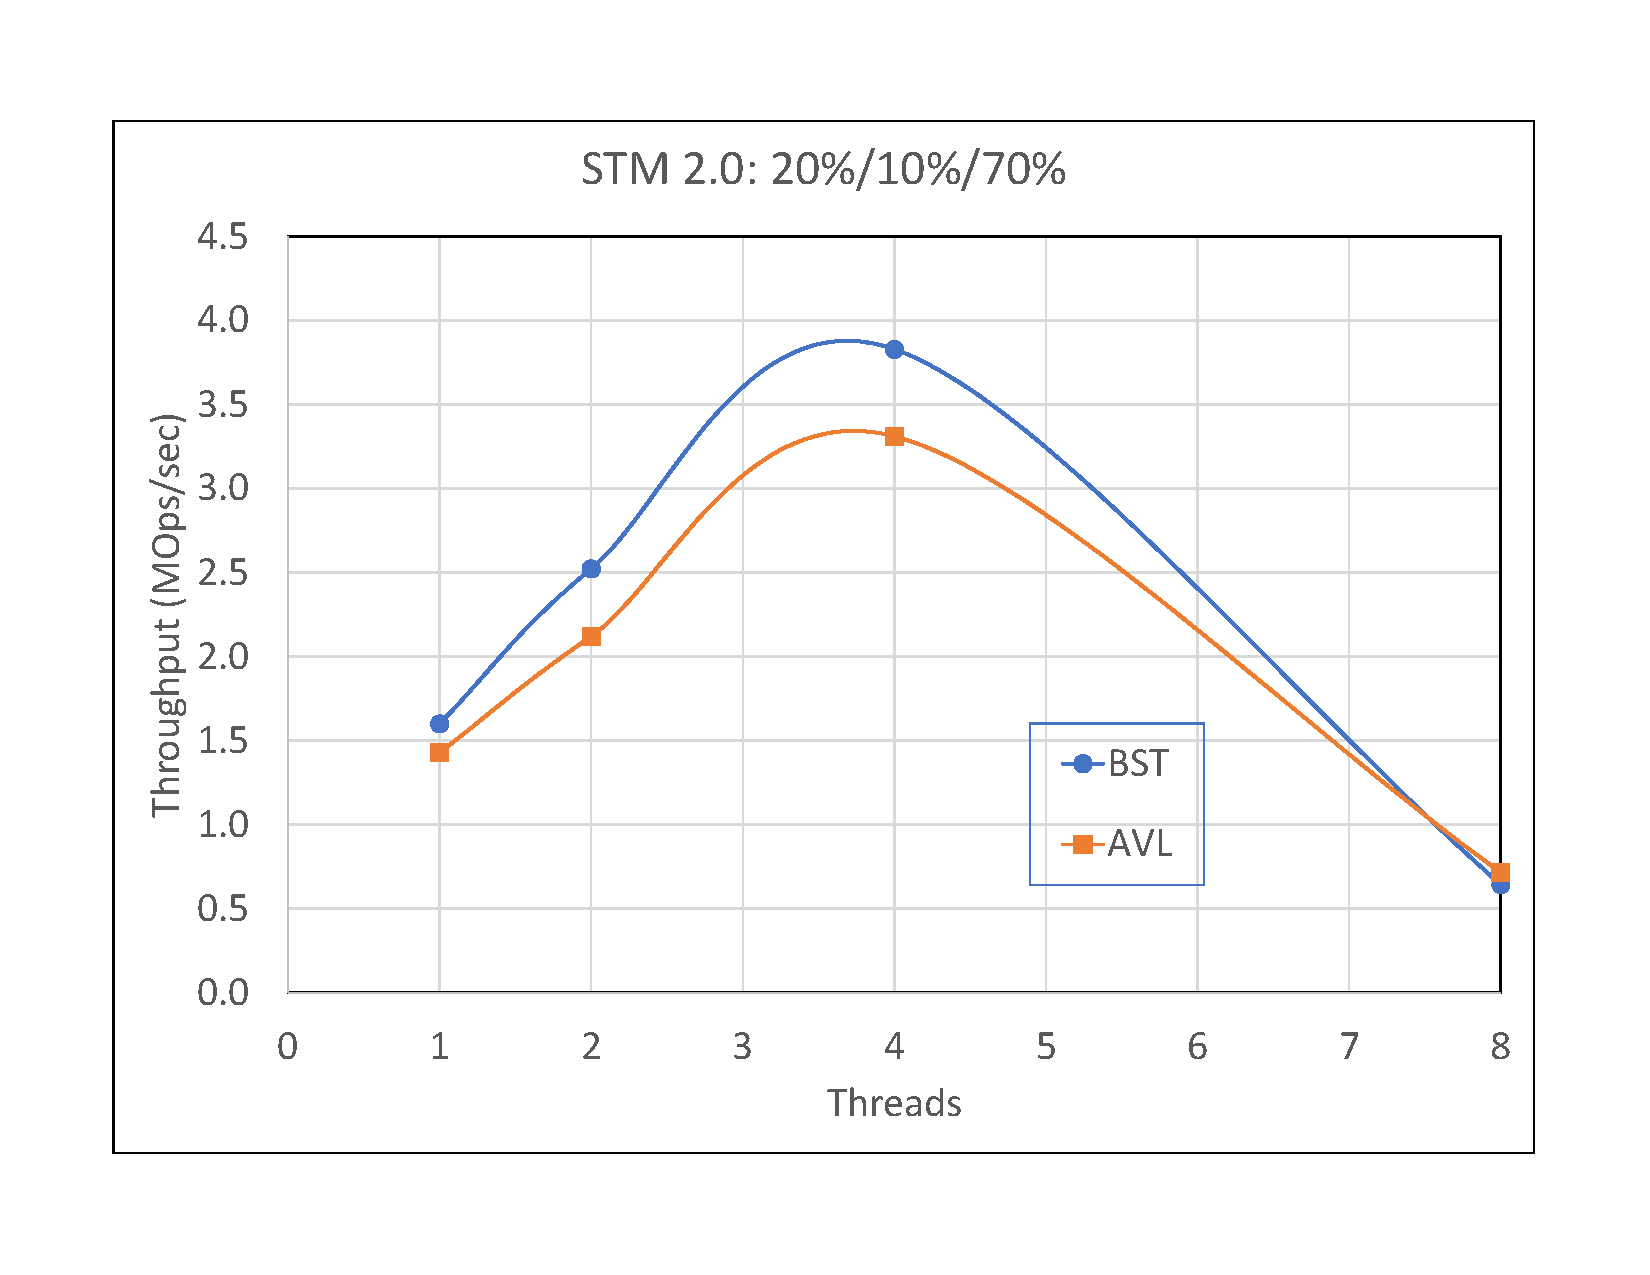
\includegraphics[width =\linewidth]{figures/stm2-20-10-70}\\
(b) \\
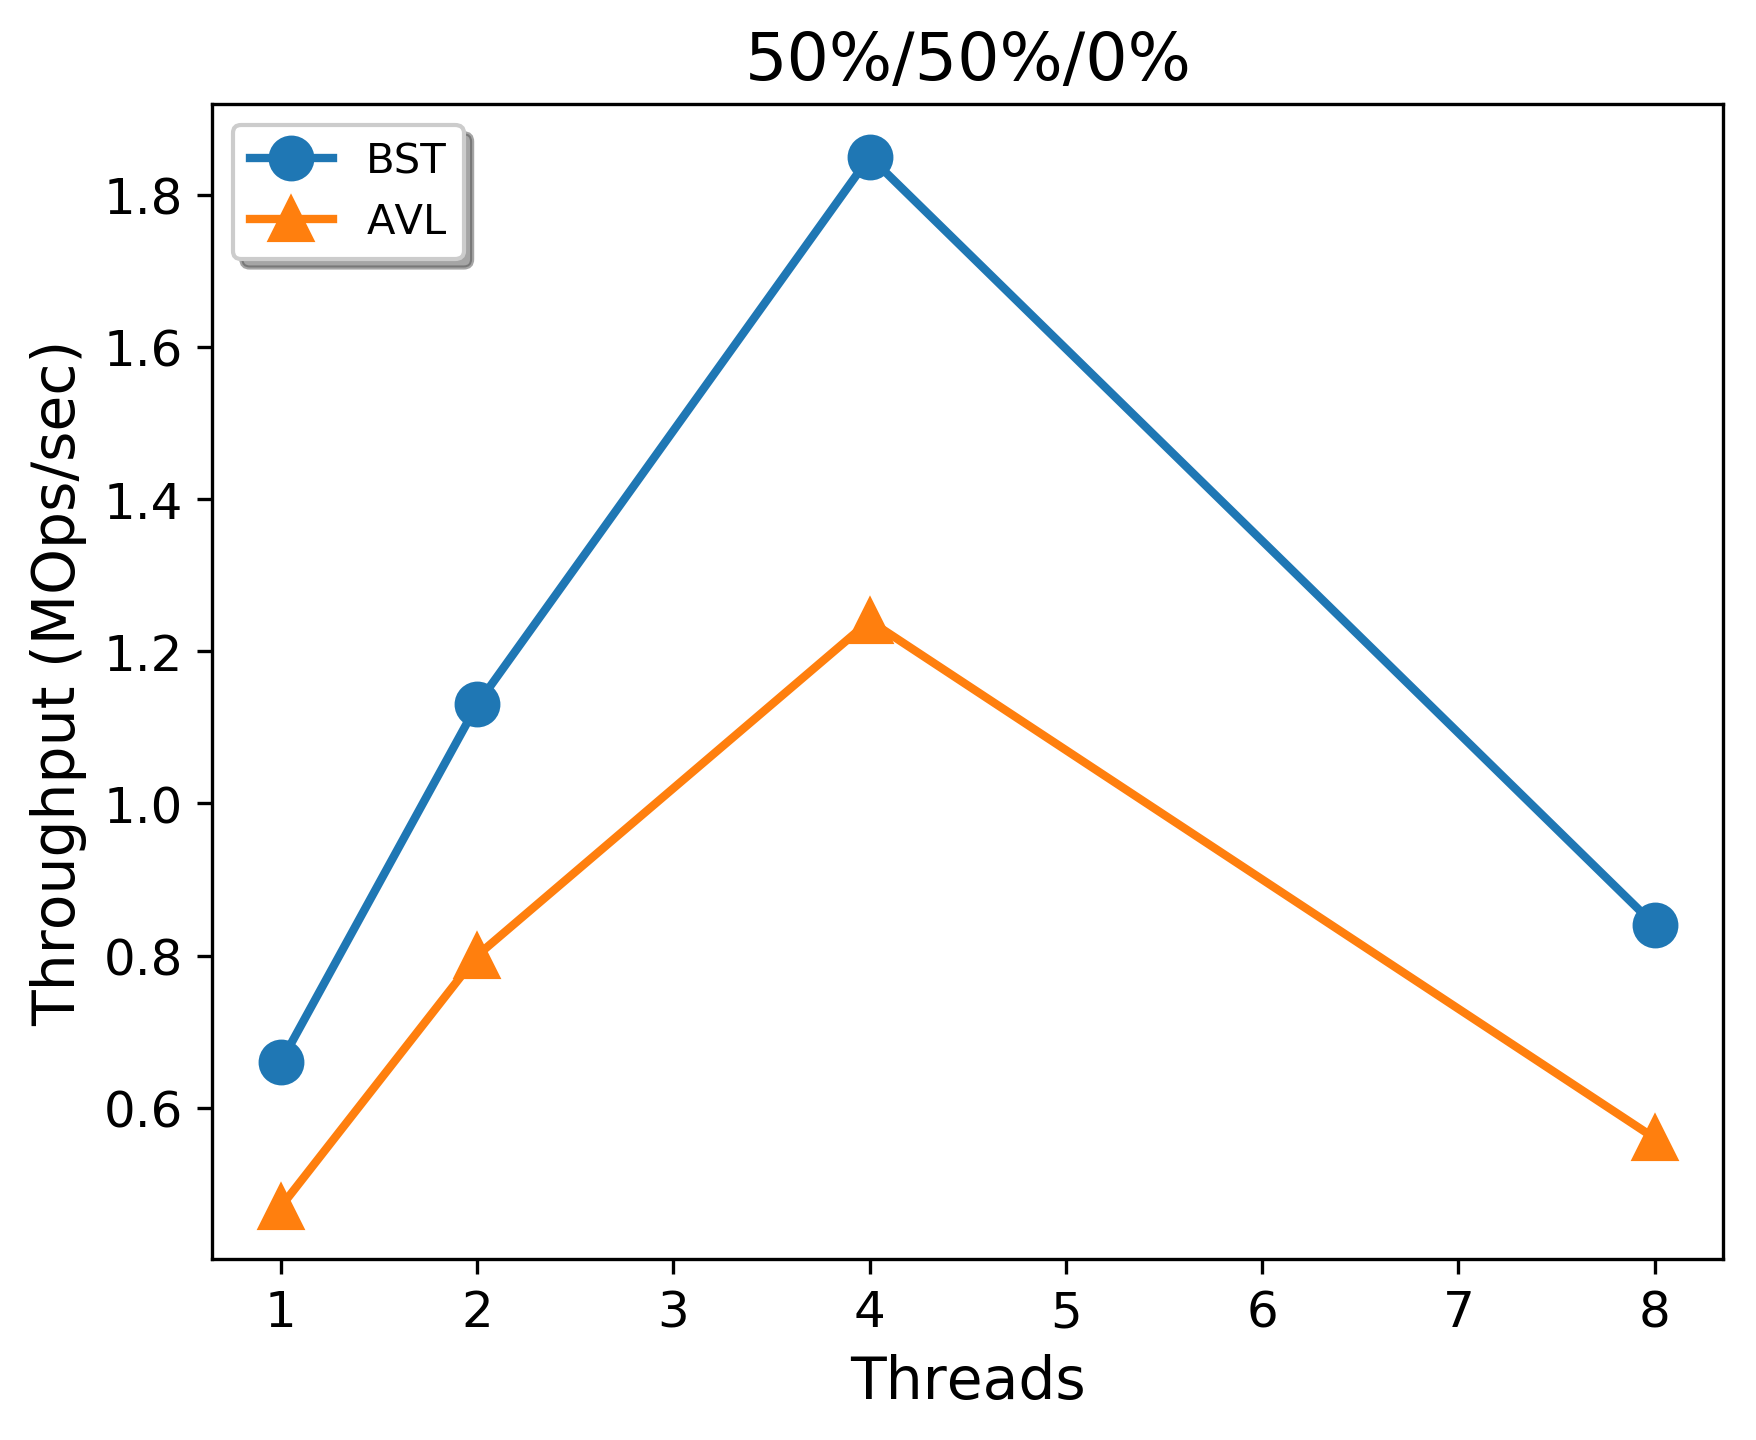
\includegraphics[width =\linewidth]{figures/stm2-50-50-0} \\
(c) 
\end{tabular}
\caption{adsf}
\end{figure*}
\fi

\section{Issues / Problems}
There are plenty of interpretations of how to go about implementing the pseudo code \cite{b1} provided by the authors, since the developed implementation left out an entire function. To start developing, first it is necessary to understand what the PaVT condition is and how can it be maintained. This was first obstacle to overcome when developing this. The redefining of how to store and maintain snapshots caused some confusion and made it hard to understand after a couple readings. Luckily, the authors have slides \cite{b3} online that increased clarity and made it possible for pushing the implementation further along the development cycle. While it was possible to develop the core of this concurrent data structure, the development of the data structure came to a halt because of one particular method. The remove function was a nightmare to program with how many locks to keep track of and ensuring the correct mutexes were locked or unlocked. This problem came from the earlier confusion of how to keep track of PaVT condition, but it more importantly it stemmed from the authors decision to leave out an important detail on what to lock in their BST remove pseudo code \cite{b1}. The deadlocks became increasingly infuriating since it seemed like the data structure will always be deadlocking, but after contacting the authors, it was possible to  gain some insight from what Drachsler-Cohen has posted and thus it solved the dilemma where the remove function needed to also lock the predecessor for the data structure to not deadlock. One major issue that might get noticed is just how many locks the remove function can use. Tracking this many locks was difficult and further portrayed just how complicated concurrent structures can be and it also proves just how useful transactional data structure can be as well, since this removed this salient roadblock all together.
\section{Discussion}
Search trees are always a relevant topic and the need for a quick and easy to maintain tree is always desired. The creation of general rules and conditions that can be applied to all can serve as a foundation to future implementations. This implementation and the authors research paper \cite{b1} displayed the power of PaVT condition. The question now is how do we improve this implementation and what else could be achievable?
\subsection{Improvements}
There are always improvements to be made since the contains itself is not wait-free and as small as it could possibly be. If more research was done as to how to reduce the size of contains and traverse while using the idea or extending the PaVT condition then it should be possible to create a data structure sought out by every programmer. One major improvement that needs to be researched is to improve remove since it is very cumbersome and blocks too many other threads from proceeding in its current state. This improvement would only be a small improvement though since remove operations are typically not called as much, but it would allow for an increasingly superior general search tree data structure.
\subsection{Other possible implementations}
As previously stated, the discovery that the authors have made is incredible since the PaVT condition can be extended to any kind of search tree. The first step to take after reimplementing a binary search tree and an AVL tree is to check and verify if this condition holds true for other types of search trees. This concurrent implementation has only verified BST and AVL trees, but trying to recreate and maintain this condition in more complicated trees, such as an m-ternary tree, might prove to be too difficult to maintain to outweigh the benefits.


\section{Appendix}

\section*{Acknowledgment}

\section*{References}

% TODO: FIX REFERENCES
%Practical Concurrent Traversals in Search Trees 
%http://webee.technion.ac.il/~idish/ftp/TransactionalLibrariesPLDI16.pdf - Transactional Data Structure Libraries
%http://webee.technion.ac.il/~idish/ftp/TransactionalLibrariesPLDI16.pdf



\begin{thebibliography}{00}
\bibitem{b1} D. Drachsler-Cohen, M. Vechev, and E. Yahav. 2018. Practical concurrent traversals in search trees. In Proceedings of the 23rd ACM SIGPLAN Symposium on Principles and Practice of Parallel Programming (PPoPP '18). ACM, New York, NY, USA, 207-218. DOI: https://doi.org/10.1145/3178487.3178503
\bibitem{b2} D. Drachsler-Cohen, M. Vechev, and E. Yahav. 2014. Practical Conccurent Binary Search Trees via Logical Ordering. http://www.cs.technion.ac.il/~yahave/papers/ppopp14-trees.pdf
\bibitem{b3} D. Drachsler-Cohen, M. Vechev, and E. Yahav. 2014. Practical Conccurent Binary Search Trees via Logical Ordering. https://pdfs.semanticscholar.org/f776/1f31061936218458163adaa019f6f59a9030.pdf (Slides)
\bibitem{b4} V. Luchangco, J. Maurer, M. Moir, H. Boehm, J. Gottschlich, M. Michael, T. Riegel, M. Scott, T. Shpeisman, M. Spear, M. Wong, "Transactional Memory Support for C++",[online document], 2013. Available: JtC1/SC22 subcommittee, http://www.open-std.org [Accessed: November 29, 2018]

\end{thebibliography}

\end{document}
